\section{Elektroplanung und Realisierung \textcolor{gray}{(Nikolaj Voglauer)}}

\subsection{Elektroplanung}
\label{sec:Elektroplanung}

\subsubsection{Einleitung - Grundanforderungen}
    Die grundsätzliche Zielsetzung bei der elektrischen Planung, war die Anforderungen so zu erfüllen, dass die Lösung einerseits die Anforderungen von Erweiterbarkeit und Mobilität erfüllen und andererseits in der Schule beziehungsweise in der Werkstätte produzierbar waren. Die Elektrik des AFSS befindet sich in einem umgebauten Serverschrank, dessen physische Limitierungen bei der Planung ebenfalls zu berücksichtigen waren. Darunter fällt beispielsweise, dass die Module in die Breite von den, nur in die Tiefe verstellbaren, Profilschienen begrenzt werden.\\
    In der Anlage sollten während dem Normalbetrieb alle Komponenten vor elektrischen Störungen geschützt sein. Der Fokus liegt hierbei auf dem Schutz von Messleitungen und Steuerleitungen, denn diese überliefern präzise Daten die nicht verzerrt werden sollen.\\ 
    In der Planung wurde stehts bedacht, dass die elektrischen Komponenten so verbaut werden, dass im Falle eines Fehlers sowohl Personen gut geschützt sind und betroffene Geräte leicht auszuwechseln sind.\\

\subsubsection{Elektrik spezififsche Anforderungen}
\label{sec:Elektrik spezififsche Anforderungen}

    \paragraph{Versogung}\mbox{}\\
    Zur Verfügung steht dem AFSS eine 3-phasige Wechselspannung mit 400V Außenleiterspannung. Damit direkt angesteuert werden kann nur der Asynchronmotor für das Fließband. Alle anderen Elemente brauchen eine andere Spannungsebene. Die, in Summe, sieben Schrittmotoren brauchen 24 V mit einem möglichen Dauersummenstrom von über 20A. Die Logik bestehend aus Siemens-SPS, mit Ein und Ausgangskarten sowie PTO-Karten, und einer ET200 mit Asi-Master. Die Logik benötigen ebenfalls 24 V und sollen getrennt versorgt werden, um von potentiellen Fehlern bei den Schrittmotoren geschützt zu sein. Der Asi-Kreis benötigt eine eigene Asi-24V-Versorgung.

    \paragraph{Ansteuerungen}\mbox{}\\
    Angesteuert werden müssen 8 Motoren: 1 Asynchronmotor (250 W), 4 stärkere Schrittmotoren (2 Nm) und 3 schwächeren Schrittmotoren (40 Ncm). \\
    Der Asynchromotor soll keine Drehzahlregelung haben und über eine Wendeschützschaltung angesteuert werden. Die Schrittmotoren sollen über Schrittmotortreiber angesteuert werden. Diese Treiber werden von den PTO-Karten der SPS angesteuert.

    \paragraph{Sicherheit}\mbox{}\\
    Für die Anlage soll ein Fehlerstromschutzschalter (FI), ein Leitungsschutzschalter (LS), ein Motorschutzschalter und für jeden Schrittmotor eine Gleichstromsicherung ausgelegt werden.\\ 
    Um die Anlage trotz Fehler, die potentiell von den elektrischen Schutzeinheiten nicht erkannt werden, nach wie vor Abschalten zu können soll die Anlage über mehrere Not-Aus-Schalter verfügen. Zwei auf der Anlage selsbt, einen im Serverschrank/Schaltschrank und einen am Kommisionierplatz. Diese Positionierung soll es NutzerInnen ermöglichen aus jeder Position an der Anlage, einen Not-Aus-Schalter zu erreichen.

    \paragraph{Bedienelemente}\mbox{}\\
    Physische Bedienelemente wären beim AFSS ein Schlüsselschalter, zur Freigabe, und ein dreiphasiger Drehstromschalter, für eine manuelle Freischaltungsoption.

    \paragraph{Schaltschrank}\mbox{}\\
    Grundsätzlich haben Schaltschränke genormte Anforderungen (IEC 60208 und IEC 61439).\\
    Dazu gehört eine Auslegung von Kabelkanäle, die die Kabel schützen soll und Umbauten nicht zusätzlich erschweren sollen. Freifliegende Kabel sollen unter allen Umständen verhindert werden. Das Gehäuse muss geerdet sein und die inneren Komponenten vor Staub und Schmutz schützen. Bei einem potenziellen Lichtbogen soll der Schaltschrank Personen in der Nähe schützen. Zudem muss der Schrank gegen thermische Einflüsse geschützt sein, gegebenenfalls soll der Schaltschrank über eine Belüftung verfügen.\\
    Der Serverschrank, für den wir uns entschieden haben, schütz gegen Staub und Schutz und kommt mit einer Lüfteranlage, die die Abwärme von mehereren Gleichrichtern gut abführen kann. Zudem sind die Materialen des Schrankes vor Korrosion geschützt. \cite{Schaltschrank-Anforderungen} \\
    Bei der Planung muss beachtet werden, dass die Erdung aller leitungsfähigen Elemente eingehalten wird. Außerdem dürfen Umbauten wie die Montage von Rädern keine der angeführten Anforderungen widersprechen.

    \paragraph{Kabelauslegung}\mbox{}\\
    Beim Auslegen von Kabeln gibt es mehrere Punkte, die beachtet werden müssen. Während Spannungsabfall bei den Längen des AFSS vernachlässigt, werden können muss besonders auf Schleppkettentauglichkeit geachtet werden. Steuer- und Messkabel müssen entsprechend geschirmt werden und abhängig vom Strom muss der Querschnitt gewählt werden. Dabei gehören die Querschnitte aber auch auf die Schutzautomaten im Stromkreis abgestimmt.\\

    \paragraph{Module}\mbox{}\\
    Die Paneele/Module, auf welchen die elektrischen Komponenten montiert werden, müssen ebenfalls alle Erdungserwartungen erfüllen und mechanisch den Belastungen standhalten. Dabei ist das Gewicht die gravierenste Belastung. Eine gerechte Verdrahtung muss gewährleistet sein und die Modularität der Paneele soll vorteilhaft ausgenutzt werden und sollen nicht das Projekt unnötig verkomplizieren. Kostentechnisch soll dabei ein möglichst billiges, aber standhaftes Material gewählt werden.

\subsubsection{Mechanische Planung}

    \paragraph{Schaltschrankrahmen}\mbox{}\\
    \begin{figure}[h]
        \centering
        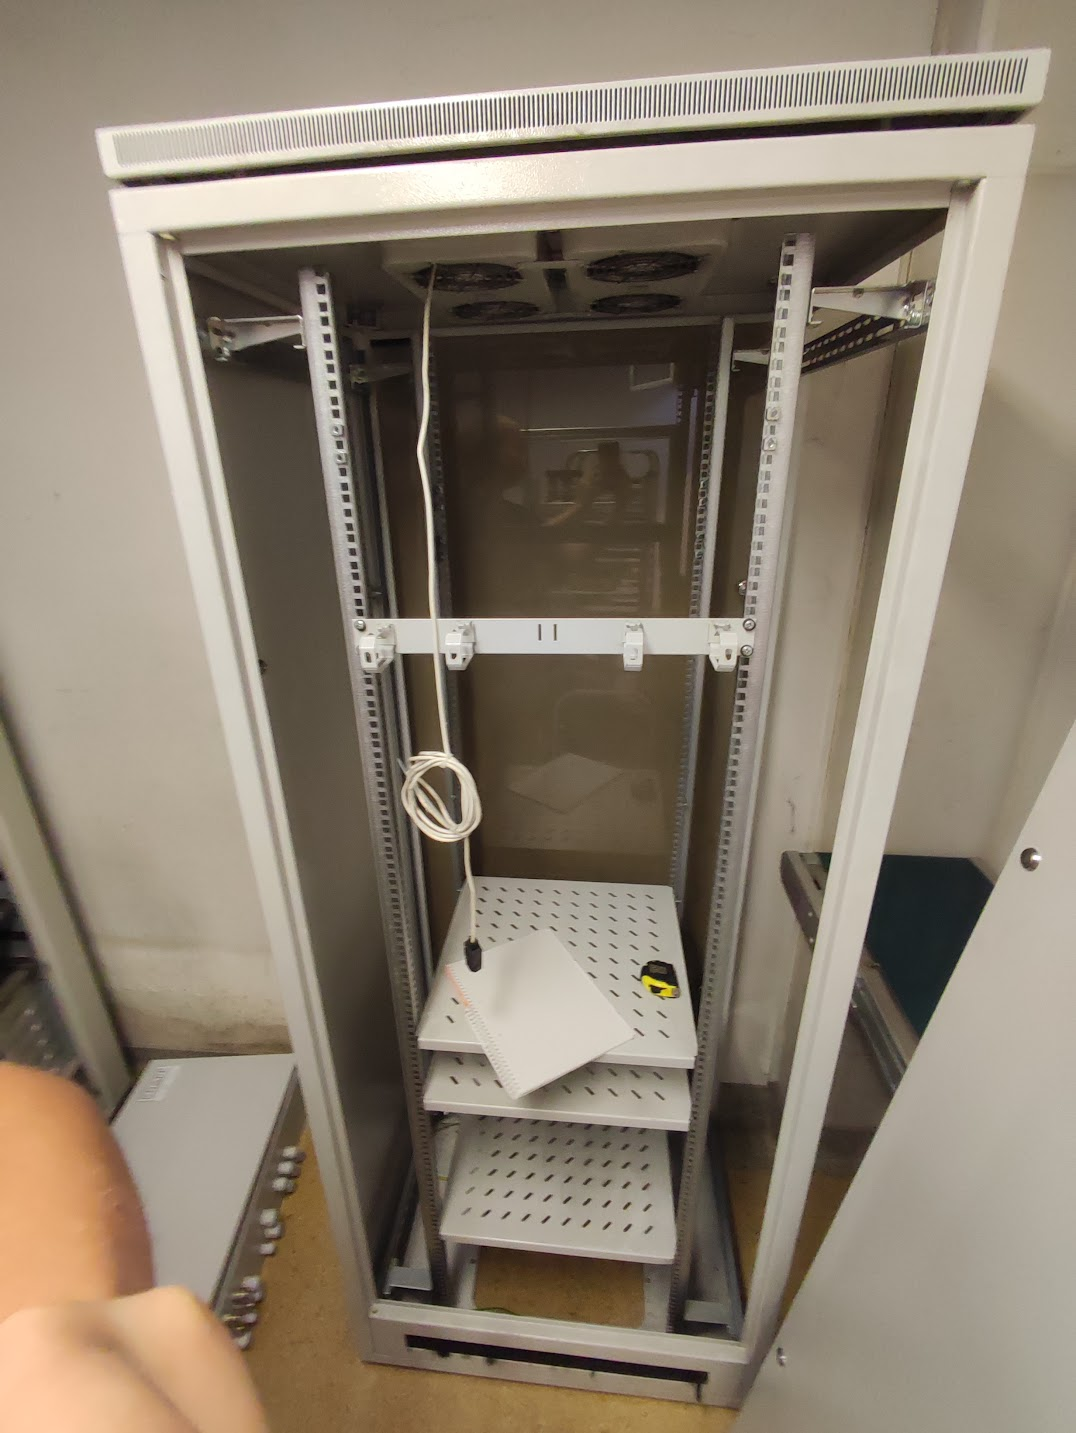
\includegraphics[width=0.5\textwidth]{Vogis Bilder/Serverschrank_original.jpg}
        \caption{Serverschrank bei Übergabe an das AFSS-Team}
        \label{fig:Serverschrank_original}
    \end{figure}
    Bevor man sich den Details des Schaltschrankes widmet, muss vorerst der Rahmen festgelegt werden. Grundsätzlich würde man einen herkömmlichen Schaltschrank verwenden, allerdings sind diese teuer und erfüllen auch nicht unsere Anforderung der Mobilität. Deswegen wurden mehrere alternative Optionen in Betracht gezogen. Anfangs wurde der Ansatz verfolgt die elektrischen Komponenten in den Lagerschrank selbst einzubauen. Dabei hätte man entweder einen eigenen Abteil ins AFSS einplanen können, der auch mittels entsprechendem Material räumlich getrennt wäre, oder man hätte die Elemente fluide unterbringen können. Mit Letzteren ist gemeint, dass in dem ganzen Schrank verteilt die elektirschen Komponenten montiert wären.\\
    Die fluide Variante benötigt sorgfälltige Planung und auch sorgfälltige Absprache mit der restlichen mechanischen Planung des AFSS. Dafür hätte man eine kompacktes Design aber das Risiko für Verletzungen und Schäden wäre höher, da man die elektrischen Komponenten nur schwer räumlich trennen könnte, so wie es die Wände eines Schaltschrankes machen. Aufbauend auf dem fehlenden Sicherheitsaspekt und der Tatsache, dass die benötigte Kommunikation in einer Entwicklungsphase nicht möglich wäre, wurde sich gegen die fluide Option entschieden.\\
    Wesendlich realistischer ist der Ansatz ein eigenes kleines Abteil in den Schrank einzubauen. Der Rahmen wäre, sowie das Lager, aus Aluminiumprofilen gebaut und die jeweiligen Seiten würden mit Kunstsoffen verkleidet werden. Um die räumliche Trennung zu gewährleisten. Diese Option wäre Kommunikationstechnisch möglich, da man sich mit der restlichen mechanischen Planung nur auf die Außenmase und Position dieses Abteils einigen müsste. Allerdings bedeutet ein intigriertes Abteil auch weniger Lagerplätze und einen merkbaren Zusatzaufwand in der Realisierung. Da so viele Lagerplätze wie möglich verwirklicht werden sollen wurde sich gegen diese Variante entschieden.\\
    Auf der weiteren Suche nach einer Alternative zum herkömmlichen Schaltschrank wurde die Möglichkeit, einen alten Serverschrank zu recyclen erkannt. Ein fertig gebauter Schrank, der im Fehlerfall die Umgebung ausreichend schützt und keine Zusatzkosten mit sich bring war die beste Option. Die im Inneneren bereits vorhandenen Profilschienen bieten viele Möglichkeiten für die Elektrik montiert zu weden. Zudem bietet der Innenraum des Serverschrankes viel Platz und auch die Möglichkeit die Elektrik, wenn nötig, zügig zu erweitern, da man die Profilschienen sehr indiviuell nutzen kann.\\
    Es wurde sich somit entschieden den Serverschrank zu einem Schaltschrank umzubauen. Im Zuge des Umbaus würde der Innenraum umgebaut werden und der Serverschrank müsste auch mobil gemacht werden. 
    \paragraph{Modulprinzip}\mbox{}\\
    Im Zuge dieses Projektes wurde das Innenleben des Schaltschrankes auf mehrere Module getrennt. Die Anforderungen an diese wurden schon beschrieben, doch ursprünglich waren weitere Alternativen für den Innenraum des Serverschrankes in Diskussion.\\
    Anstatt von mehreren Modulen, die später genauer beschrieben werden, könnte man eine durchgehende Platte verwenden und diese an die Profilschienen des Serverschrankes festschrauben. Der große Vorteil einer durchgehenden Platte ist, man könnte die Elemente so anordnen, dass die Fläche von Leerräumen  minimiert wird. Die große Platte entfällt als Möglichkeit allerdings insofern, da diese nicht in der Schule produzierbar gewesen wäre.\\
    Eine andere Option wäre eine plattenlose, dabei würde man die Hutschienen direkt auf die Profilschienen des Serverschrankes montieren. Man spaart sich so eine Platte und die Elemente könnten direkt auf die Hutschienen montiert werden.
    Die plattenlose Option wäre eine kosteneffiziente Möglichkeit, allerdings gibt es viele Elemente, die im Schaltschrank nicht auf Hutschienen montiert werden können, diese bräuchten immer eine Montageplatte.\\
    Damit ein einheitliches Design eingehalten werden kann, wurde sich für ein Modulprinzip entschlossen. Dieses ermöglicht es allen Elementen, auch für die, die für Hutschienen ungeeignet sind, montiert zu werden und ist dennoch in der Schule produzierbar.

    \paragraph{Platten-Material}\mbox{}\\
    Für die Materialwahl gab es drei realistische Möglichkeiten. Die Modulplatten hätten vollständig aus Aluminium oder aus Dibond gefräst werden können. Als dritte Option hätte man die Platten aus einem Kunststoff lasern oder fräsen können. Die Aluplatten bieten den Vorteil der Leitfähigkeit und somit müsste man nur die Platte erden und die Elemente auf der Platte wären alle dementsprechend geerdet. Beim einer reinen Kunststoffplatte gibt es keine Leitfähigkeit und zusätzlich bieten die meisten Kunststoffe keine ausreichende mechanische Stabilität.\\
    \begin{figure}[h]
        \centering
        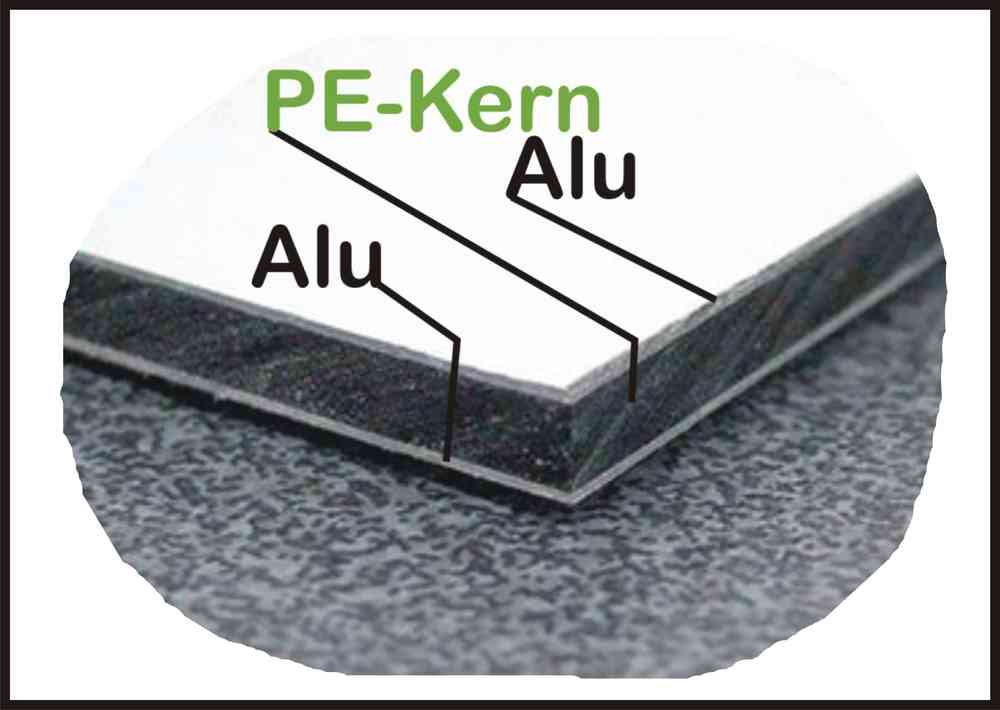
\includegraphics[width=0.5\textwidth]{Dibond_Platten_ml.jpg}
        \caption{Dibond-Platte, Quelle: \cite{Dibond-Platte}}
        \label{fig:Sommerprototyp}
    \end{figure}  
    Aluminium erfüllt alle Anforderungen, ist aber teuer und ein wertvoller Werkstof. Da ein umsichtiger Umgang mit Ressourcen wichtig ist wurden nach einer Alternative gesucht. Dibond wurde daraufhin als Projektstandard für die Module definiert. Dieser Stoff besteht aus zwei dünnen Aluminiumplatten die auf einen Kunststoff aufgepresst werden. Dibond bietet keine elektrische Leitfähigkeit, folglich müssen alle Elemente zusätzlich geerdet werden aber das leichte Gewicht und die hohe mechanische Stabilität machen Dibond zur besten Option.

    \paragraph{Digitaler Zwilling}\mbox{}\\
    Moderner Schaltschrankherstellung begegnen im Herstellungsprozess oft große logistische Probleme. Jeder Prozessschritt ist eine Fehlerquelle und wenn Fehler nicht früh erkannt werden, pflanzen sich diese fort. Damit zwischen den Prozessschritten keine Kommunikationsprobleme entstehen setzen viele Hersteller auf das Prinzip des digitalen Zwillings.\\
    Dieser ist im Grunde ein digitaler Schaltschrank, welcher im ersten Prozessschritt, der Planung, ausgeplant wird und im Herstellungsprozess, sei es der Schrankbau oder die Bestückung, wird einerseits immer derselbe digitale Zwilling aktualisiert und aber auch referenziert. Das heißt alle Prozessschritte beziehen sich auf denselben Plan bzw. digitalen Zwilling (siehe \ref{fig:digilaerZwilling}).
    \begin{figure}[h]
        \centering
        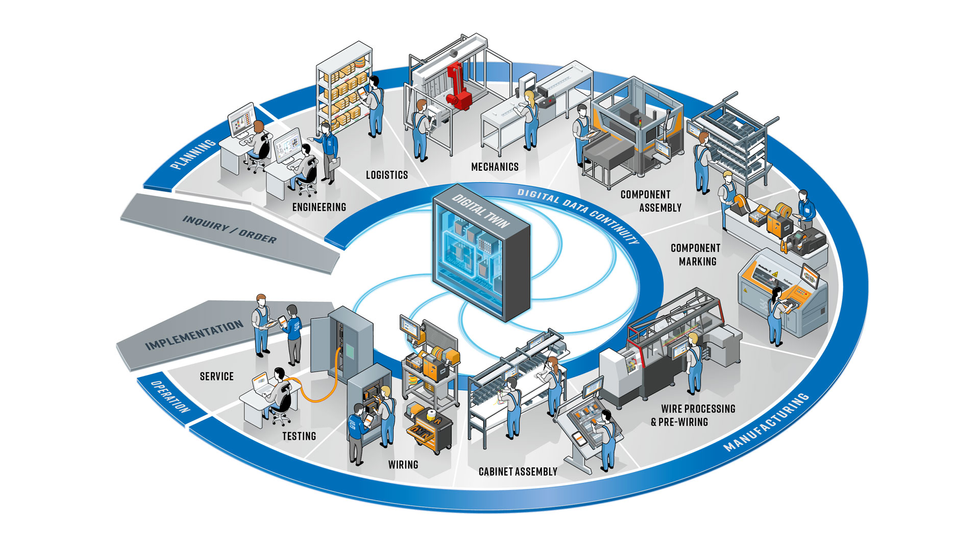
\includegraphics[width=0.9\textwidth]{Cabinet-Building-Komax-SCB-Component-Printer.png}
        \caption{Digitaler Zwilling, Quelle: \cite{digitaler_zwilling_bild}}
        \label{fig:digilaerZwilling}
    \end{figure}
    Es setzt auch ein breites Feld an Firmen auf dieses Prinzip. Firmen wie Weidmüller, Komax, Steinhauer und noch viele mehr haben eine Firmenzusammenarbeit, die ohne einen digitalen Zwilling nicht möglich wäre \cite{smart_cabinet_building}. In diesem Fall werden die jeweiligen Prozessschritte meistens von einer neuen Firma übernommen. In diesem Bündnis ist der digitale Zwilling der Schlüssel zum Erfolg. Man kann dieses Prinzip der Dokumentation bzw. Planung als Industriestandard verstehen.\\
    Um den Prozess der Herstellung des Schaltschrankes möglichst nahe an die Praktiken aus der Industrie anzugleichen, wird auch der Schaltschrank des AFSS mithilfe eines digitalen Zwillings geplant. Dieser wird in Fusion360 gezeichnet und soll den Sollzustand des Schaltschrankes abbilden.\\
    Um die Konstruktion anzufangen, braucht es eine möglichst ausführliche Ausmessung des bereits bestehenden Serverschrankes. Besonders wichtig sind die Elemente die direkt am Umbau beteiligt sind, wie die Profilschienen (Abstände der Löcher, Abstände der Profilschienen zueinander und detaillierte Abmessungen der Profilschienen selbst.), die Türen und die Lüfter.\\

    \paragraph{Digitaler Zwilling - Umsetzung}\mbox{}\\ 

    \begin{figure}[h]
        \centering
        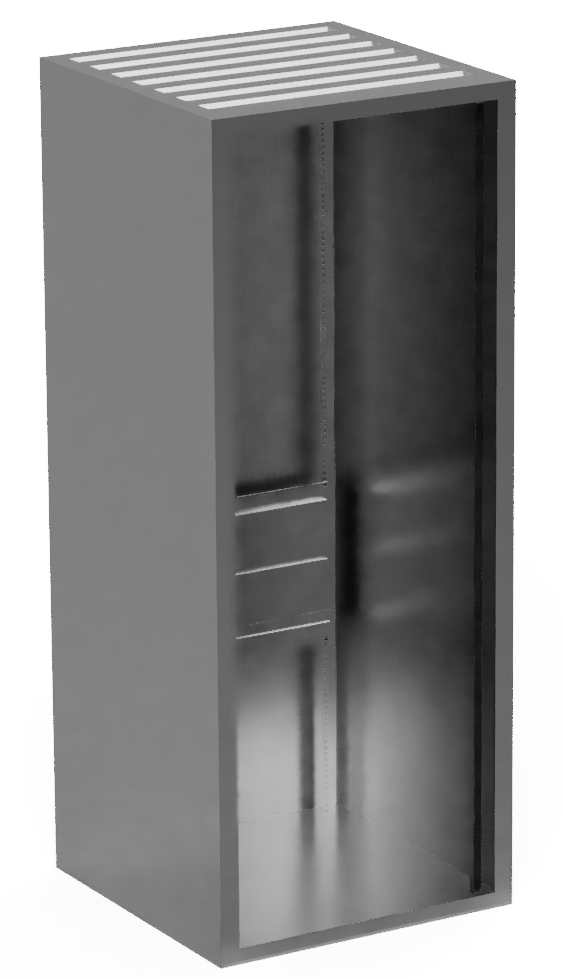
\includegraphics[width=0.3\textwidth]{Prototyp_Serverschrank.PNG}
        \caption{Sommerprototyp eines Serverschrankes}
        \label{fig:Sommerprototyp}
    \end{figure}
    Als Erstes muss der Serverschrank, wie bereits erwähnt ausführlich ausgemessen werden. Äußere Höhe, innere Höhe, Äußere Breite, innere Breite und noch Vieles mehr muss richtig gemessen werden.    
    Bei den Messungen werden Messschieber und bei größeren Abständen Maßbänder verwendet. Um die mechanische Konstruktion zu erleichtern, werden alle Daten digital festgehalten.   
    Während die Messungen des Serverschranks für den finalen digitalen Zwilling wichtig werden, gibt es aber auch noch andere Punkte, beispielsweise bestand lange die Frage, ob das Modulkonzept so möglich sei. Aufgrund dessen und des Umfanges der Diplomarbeit sowie der begrenzten Zeit wird ein erster Entwurf eines Serverschrankes in Fusion360 konstruiert und weiters ein Probemodul gezeichnet. Die Maße dieses digitalen Prototyps sind von einem Standard-Serverschrank aus dem Internet übernommen.
    Dieser Prototyp hat nicht dieselben Werte wie der richtige Serverschrank, der dem AFSS zur Verfügung steht. Aufgrund der Prototyp-Konstruktion steht fest, dass das Modulkonzept ist so umsetzbar. Weiterführend ist festgestellt, wie man optimierter in Fusion Zeichnen kann.
    Eine Erkenntnis des Prototyps ist, dass man den Serverschrank nicht als ein großes Element konstruieren sollte, da wenn ein Fehler spät erkannt wird dieser so gut wie nicht mehr zu beheben ist. Wenn die Konstruktion allerdings auf viele verschiedene Elemente aufgeteilt wird, dann ist der Schaden bei einem Fehler begrenzt. 

    Nachdem das Grundprinzip erfolgreich konstruiert wurde, ist der Serverschrank auf Grundlage der echten Maße zu konstruieren. Die gelernten Erkenntnisse werden dabei bestmöglich miteinbezogen.\\    
    \begin{figure}[h]
        \centering
        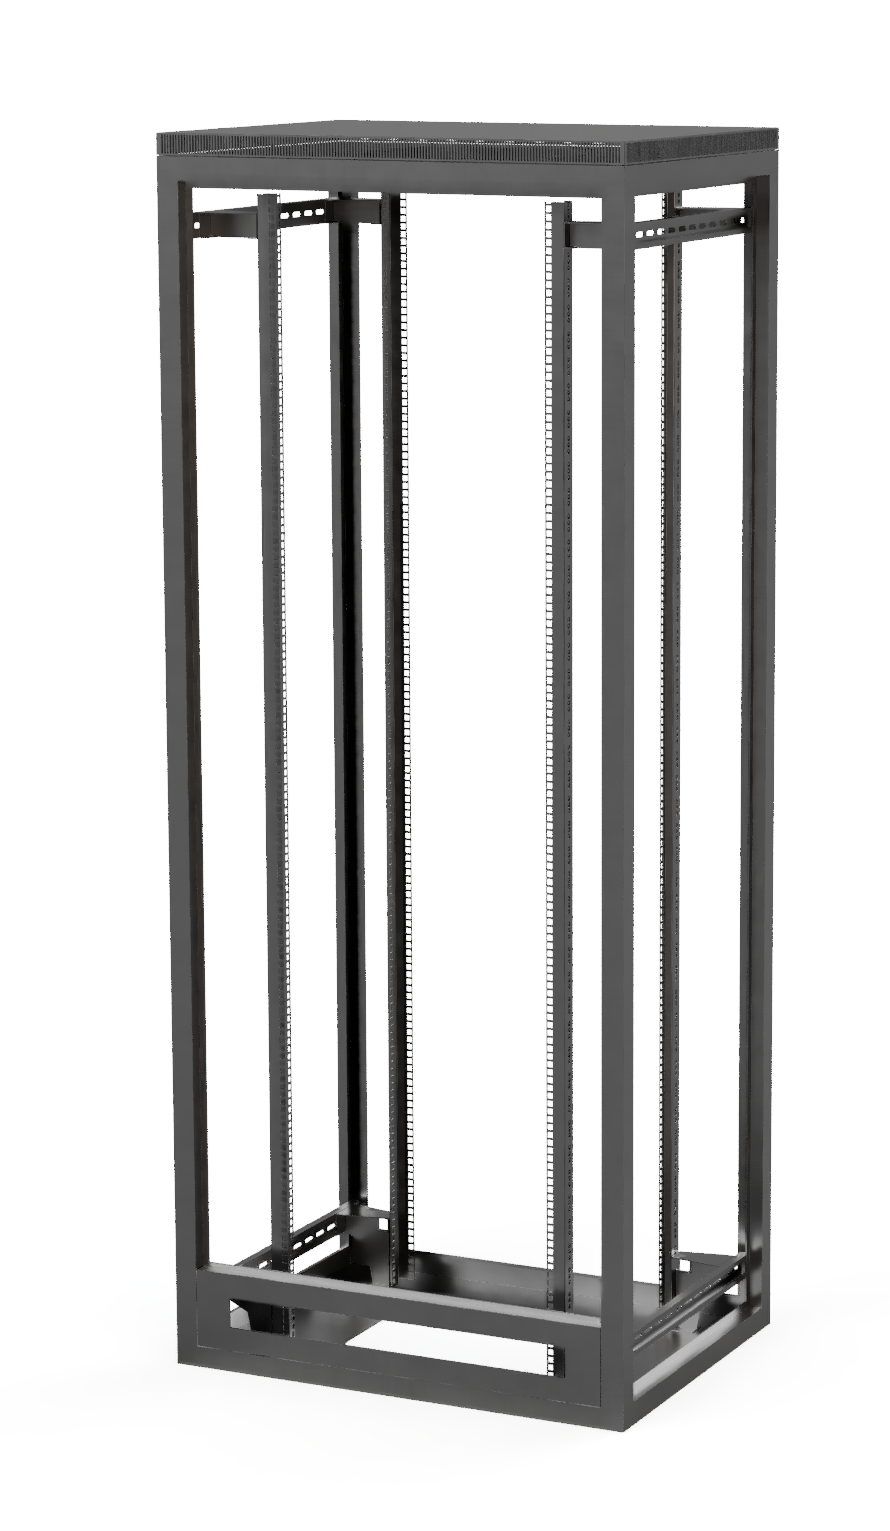
\includegraphics[width=0.35\textwidth]{Schaltschrank_ohne_Module.PNG} 
        \caption{Serverschrank konstruiert}
        \label{fig:Clean_Serverschrank}
    \end{figure}

    Mit dem fertig konstruierten Serverschrank, kann dann die Planung der Module beginnen. Dafür wird vorerst ein Konzept erstellt. Durchgedacht wird welche elektrischen Baugruppen wo im Schaltschrank platziert werden sollen. Das Konzept richtet sich einerseits nach der Vorgabe, zusammengehörige elektrische Komponenten sollen auf dasselbe Modul kommen, und andererseits zusammenhängende Module sollen sich möglichst nahe sein. 
    \paragraph{Modul 1 - Bedienelemente}\mbox{}\\
    Es sollen im Schaltschrank ein Notaus, ein Schlüsselschalter und ein Drehstromschalter verbaut werden. Diese Elemente werden gemeinsam auf einem Modul verbaut, da sie alle Bedienelemente sind.
    \paragraph{Modul 2 bis 3 - Schutzorgane und Versorgungen}\mbox{}\\
    Direkt unter dem Drehstromschalter sollen die Schutzorgane liegen. Da der Leitungsschutzschalter und der Fehlerstromschutzschalter wenig platz benötigen, werden auf dem 2. Modul zusätzlich die zwei Gleichrichter verbaut die auf eine Huttschiene montierbar sind. Damit besteht das 2. Modul aus den Schutzorganen und den Gleichrichtern. Auf die Platte muss damit auch eine durchgängige Huttschine und ein Verdrahtungskanal geplant werden.\\
    Für die reguläre Versorgung des AFSS werden drei normale Gleichrichter benötigt. Der dritte, der Deutronic Gleichrichter, kann nicht auf eine Hutschine montiert werden und hat zudem einen großen Platzbedarf. Dieser wird auf einem eigenen Modul verplant. In den Leerräumen des 3. Moduls werden Hutschinen mit Reihenklemmen verplant. Diese Reihenklemmen sollen für eine übersichtliche Verdrahtung der Versogungsleitungen sorgen.
    \paragraph{Modul 4 - ASI-Elemente}\mbox{}\\
    Konzepttechnisch ist das 4. Modul ein Erweiterungsmodul. Nur eine Ein/Ausgangsbaugruppe von Weidmüller ist auf eine kleine Huttschine verplant gewesen und der restliche Platz sollte freigelassen werden für potentielle Erweiterungen.\\
    Im Entwicklungsprozess ist deutlich geworden, dass die PWM-Signalerzeugung, der Ausgangsbaugruppen, nicht fähig sind ein veränderbares PWM-Signal zu erzeugen. Damit werden diese Elemnte nicht mehr benötigt. Parallel ist verstanden worden, dass es eine getrennte 24V-Versorgung für den ASI-Kreis geben muss. Deswegen ist im ursprünglichen Erweiterungsbereich dieses Modules, ein 24V-ASI-Gleichrichter verplant, der keine Huttschiene benötigt, und anstatt der Weidmüllerkomponenten kommmt eine ET200, an die ein ASI-Master angeschlossen ist. Zudem ist auch ein Verdrahtungskanal nötig.
    \paragraph{Modul 5 - SPS und Sicherungen}\mbox{}\\
    Das 5. Modul beinhaltet die Siemens SPS und die gesammten DC-Sicherungen für die Schrittmotoren. Für die SPS muss eine Siemens-Profilschiene auf die Platte und für die Sicherungen eine durchgängige Huttschiene und einen Verdrahtungskanal.
    \paragraph{Modul 6 - Schrittmotoren}\mbox{}\\
    Für die stärkeren Schrittmotoren werden Treiber verwendet die direkt auf einen Untergund montiert werden müssen. Die vierTreiber werden auf eine eigene Platte montiert. Auch auf diesem Modul ist ein Verdrahtungskanal nötig.
    \paragraph{Modul 7 - Ausgangsmodul}\mbox{}\\
    Am Ausgangsmodul soll einen Verdrahtungskanal haben und eine durchgängige Huttschiene. Auf diese Hutschine kommen Elemente wie die Motorschütz, Relais, die Treiber für die schwächeren Schrittmotoren und eine ausführliche Menge an Reihenklemmen.
    \paragraph{Modul 8 - Erdungsmodul}\mbox{}\\
    Etwaige Kabel des AFSS haben einen Schrim der geerdet gehört. Deswegen ist eine Erdungsplatte nötig die aus leitfähigen Aluminium gemacht werden soll. Auf dieser ist eine Ankerschiene zur Erdung von Leiterschirmen geplant. Zudem sollen in dieses Modul vier rechteckige Ausfräsungen gemacht werden, in welche die Buchse des RJ45-Stecker hineinpasst.
    \begin{figure}[h]
        \centering
        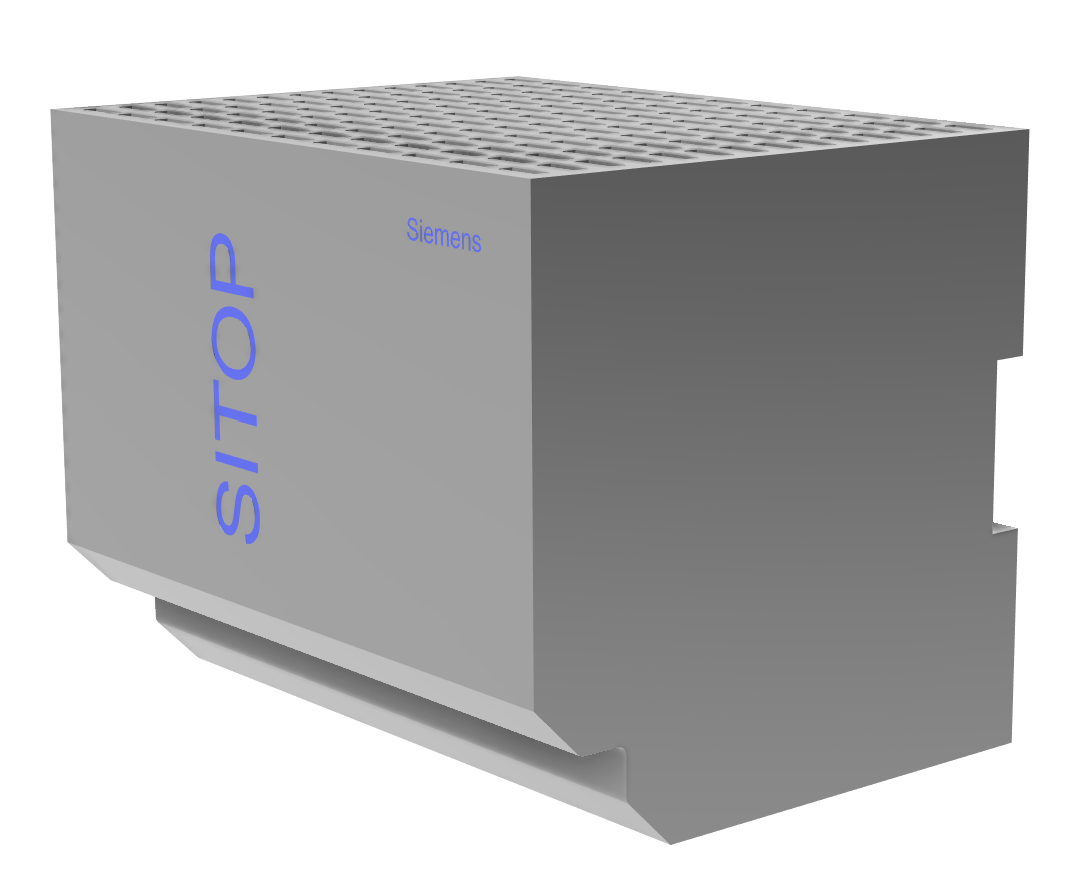
\includegraphics[width=0.3\textwidth]{Vogis Bilder/SITOP_Konstruiert.png}
        \caption{Siemens SITOP in Fusion360}
        \label{fig:SITOP_Konstrueiert}
    \end{figure}
    \paragraph{Module - 3D Konstruktion}\mbox{}\\
    Die einzelnden Module wurden, nachdem die Konzeptionierung beendet wurde, in Fusion360 gezeichnet. Dafür wurden zuerst die einzelnden Komponenten wie Hutschinen, Verdrahtungskanäle, Gleichrichter und alle anderen Komponenten als unabhängige Konstruktion gezeichnet. Damit wurde eine breite Bibliothek an Komponenten erstellt, mit dieser kann man dann wesentlich einfacher den digitalen Schaltschrank bestücken. Bei den jeweiligen Elementen ist es nicht wichtig kleinere Details miteinzubeziehen, vielmehr die Außenmase und die Positionen von Montagelöchern oder des Klemmmechanismuses für die Hutschiene sollen akkurat abgebildet sein (siehe \ref{fig:SITOP_Konstrueiert}).
    \begin{figure}[h]
        \centering
        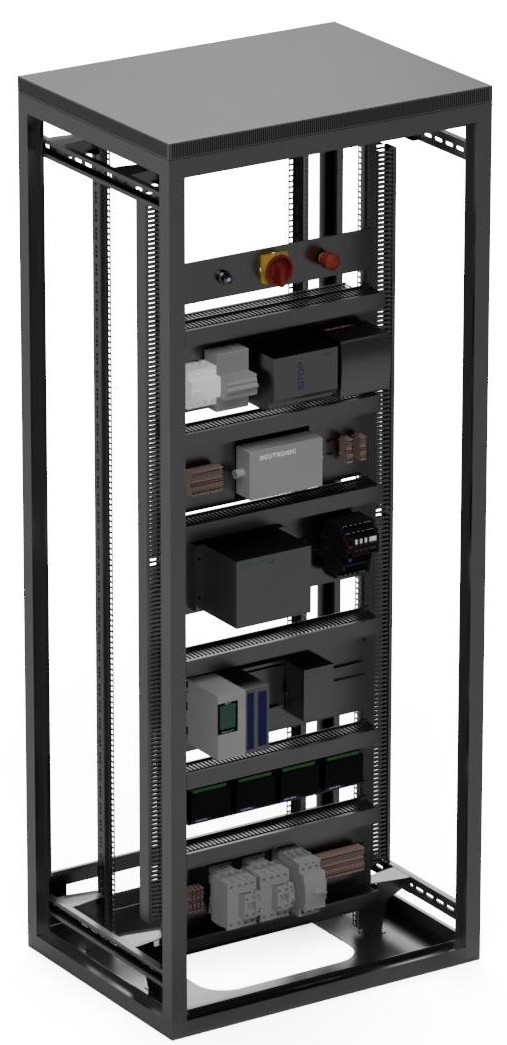
\includegraphics[width=0.4\textwidth]{Vogis Bilder/Bestuekter_Schaltschrank_Fusion.jpg}
        \caption{Der Schaltschrank in Fusion gezeichnet}
        \label{fig:Schaltschrank_bestueckt_Fusion}
    \end{figure}
    \paragraph{Fusion 360}\mbox{}\\
    Nachdem man die einzelnen elektrischen Komponenten gezeichnet hat, wurde in Fusion die erste Platte gezeichnet. Hierbei muss man nicht direkt die richtige Größe einschätzen, da Fusion späte Änderungen gut zulässt. Nachdem man eine Platte im Serverschrank konstruiert hat, kann man die Hutschienen und Verdrahtungskanäle einfügen. Daraufhin kann man die Unterkonstruktion bestücken. Beim Einfügen von Konstruktionen in andere Konstruktionen bleiben die kopierten Elemente mit der originalen Zeichnung verknüpft. Diese Verknüpfung wurde bei den Elemten gelassen, die keine Änderungen erwarten doch bei Komponenten wie eines Verdrahtungskanals sollte man die Verknüpfung trennen um das Element zuschneiden zu können. Eine Verknüpfung bedeutet, dass Veränderungen nur in der ursprünglichen Zeichnung getätigt werden können. So wurde Modul nach Modul ausgeplant.\\
    Beim Zeichnen fiel auf, dass die Module aus dem Serverschrank, beziehungsweise Schaltschrank, rausragten. Es wurde erkannt, dass die Profilschienen nach innen verschoben werden müssen um zu ermöglichen, dass sich die Wände des Schaltschrankes auch schließen lassen. Die Bauart des Serverschrankes erlaubt eine solche Veränderung.\\ 
    Es wurden, bis auf das Erdungsmodul, alle Module auf diese Art konstruiert. Man konnte schön erkennen welche Reihenfolgen sinnvoll sind und wie sich welche Komponenten am besten montieren lassen können. Beispielsweise wurde ausgetestet ob bei gewissen elektrischen Komponenten eine vertikale Montage zielführend waren. In der Abbildung \ref{fig:Schaltschrank_bestueckt_Fusion} sieht man die fertige Konstruktion des Schaltschrankes.\\
    Zu dieser Version des Schaltschrankes ist zu sagen, dass ab der Realisierung des Geplanten, dieser digitale Plan sich fließend transformiert, zum digitalen Zwilling. Dieser Zwilling gehört nach der Realisierung konstant gepflegt. Das Erdungsmodul beispielsweise, welches erst mitten in der Realisierung eingeplant und gemacht wurde, muss in den digitalen Zwilling nachträglich hinzugefügt werden.
    \paragraph{AutoCAD}\mbox{}\\
    \label{AutoCAD}
    Nachem der digitale Plan/Zwilling vollständig ausgeplant wurde, mussten die jeweiligen Platten gefräst werden.Um die Platten auch fräsen zu können müssen diese zuerst als DXF-Datei in Filou-NC eingefügt werden. Dazu mussten die einzelnen Module in AutoCAD nachgezeichnet werden.     
+
    Idealerweise hätte man hierfür nur die Oberfläche der Platten in Fusion zur Skizze gemacht und diese dann als DXF exportiert. Bei einem nachträglichen Ausmessen der 3D-Konstruktion wurde allerdings festgestellt, dass sich die Maße der Löcher der Profilschiene nicht mit der Realität decken. Zudem wurden weitere minimale Abweichungen festgestellt. Keiner der Fehler war so gravierend, dass man die digitale Konstruktion des Schaltschrankes nicht weiterverwenden könnte aber für eine präzise Fräsung aufbauend auf der Fusion-Konstruktion waren die Abweichungen zu groß. Deswegen wurden alle Module in AutoCAD sorgfälltig nachgezeichnet.\\     
    Beim Nachzeichnen wurden alle fehlerhaften Mase ausgebessert. Mit den richtigen Masen wurde festgestellt, dass sich gewisse Module nicht wie geplant ausgingen. Beim Modul 6 gingen sich die vier Schrittmotortreiber nicht vertikal nebeneinander aus. Deswegen wurde in AutoCAD einer der Treiber vertikal angeordnet und weiterführend wurde die Änderung auch in Fusion nachgebessert.
    \paragraph{Räder}\mbox{}\\
    In der Transformation vom Serverschrank zum Schaltschrank des AFSS gehört auch, dass der Schrank mobil gemacht wird. Dazu wurden zwei flexible und zwei starre Räder zur Verfügung gestellt. Planungstechnisch wurden diesbezüglich besprochen, dass die Räder direkt an das bestehende Gerüst geschraubt werden. Montiert werden die Räder mit simplen Schrauben und Muttern. Die Räder wurden in AutoCAD nicht gezeichnet, da es keinen sinnerfüllten Zweck gab. 
    \newpage
\subsubsection{Die elektrischen Komponenten}
\label{sec:Die elektrischen Komponenten}
    Das AFSS verfügt über eine große  Bandbreite von elektrischen Komponenten. Jede Art von Elementen ist zur besseren Verständlichkeit kurz aufgelistet, bevor im nächsten Kapitel die jeweiligen Funktionen beleuchtet werden.
    \paragraph{Übersicht der Komponenten}\mbox{}
    \begin{table}[h!]
        \centering
        \begin{tabular}{|l|l|c|}
            \hline
            \textbf{Allgemeine Bezeichnung} & \textbf{Typenbezeichnung} & \textbf{Funktion} \\ \hline
            Trennschalter & / & Manuelle Trennung vom Netz \\ \hline
            Schlüsselschalter & / & Freigabeschalter \\ \hline
            Not-Aus-Schalter & / & Manueller Not-Aus \\ \hline
            Motorschutzschalter & / & Schutz für ASM \\ \hline
            FI & TYP A 30mA & Fehlerstromschutzschalter \\ \hline
            LS & C13 & Leitungsschutzschalter \\ \hline
            Telemecanique & TSX-SUP-A054 & 400/24V ASI-Netzteil \\ \hline
            SITOP & 6EP1436-3BA00-8AA0 & 400/24V Netzteil \\ \hline
            Deutronic & DP500IP/3-24 & 400/24V Netzteil \\ \hline
            Meanwell-Netzteil & DRT-240-24 & 400/24V Netzteil \\ \hline
            Telemecanique & TSX-SUP-A054 & 400/24V ASI-Netzteil \\ \hline
            SPS & 6ES7515-2AN03-0AB0 & Steuereinheit \\ \hline
            SPS-DI-Karte & 6ES7521-1BL00-0AB0 & Digitale Eingänge \\ \hline
            SPS-DO-Karte & 6ES7522-1BL01-0AB0 & Digitale Ausgänge \\ \hline
            SPS-PTO-Karte & 6ES7553-1AA00-0AB0 & Erzeugung von PWM-Signalen \\ \hline
            ET 200 SP& 6ES7155-6AU01-0CN0 & dezentrale Peripherie \\ \hline
            ET 200 Busadapter & 6ES7193-6AR00-0AA0 & Busanschluss \\ \hline
            ET 200 ASI Master & 3RK7137-6SA00-0BC1 & ASI-Master \\ \hline
            ET 200 Steckadbater & 6ES7193-6BP20-0DC0 & Steckadapter für ASI-Master \\ \hline
            ASI-Slaves & 3RK2200-0CE02-0AA2 & Nimmt Sensoren auf \\ \hline
            Feed-In-Modul & 2081870000 & Eingang zu DC-Sicherungen \\ \hline            
            Service Schnittstelle & IE-FC-SET-SPDEK001-KY-P & Schnittstelle für externen Zugriff \\ \hline
            8A-DC-Sicherung & 2080600000 & Sicherung von SM \\ \hline
            2A-DC-Sicherung & 2080480000 & Sicherung von SM \\ \hline
            SM-Treiber groß & CL57T(V4.0) & Ansteuerung von SM \\ \hline
            SM-Treiber klein & TB6560 & Ansteuerung von SM \\ \hline
            SM 2Nm & 23E1K-20 & Antrieb X und Y Achse \\ \hline
            SM 40Ncm & 17HS4417P1-X4 & Antrieb für Gabel und Querförderer \\ \hline
            ASM & Spörk Antriebssysteme & Antrieb für Förderband \\ \hline
        \end{tabular}
        \caption{Übersicht der elektrischen Komponenten}
        \label{tab:elektrische_komponenten}
    \end{table}
\subsubsection{Elektrische Planung (E-Plan)}
\label{sec:Elektrische Planung}
    Für das Zeichnen eines E-Plans ist ein großes Produktwissen nötig. Um sich dieses zu beschaffen wurde die mechanische Seite zuerst geplant, da man im  Zuge dieser die elektrischen Komponenten sehr gut kennenlernt. Als ein großteil der mechanischen Seite für den Schaltschrank ausgeplant war wurde der E-Plan parallel zur mechanischen Planung angefangen. Als Schüler wurde die E-Plan Education Version verwendet. Diese Version ist kostenlos und bietet alle Funktionen die für die Planung des AFSS nötig sind.
    \paragraph{E-Plan Allgemein}\mbox{}\\
    Die Firma E-Plan bietet verschiedenste Möglichkeiten zur Planung und Dokumentation von elektrischen Anlagen. Das Programm bietet auch die Möglichkeit eines Aufbauplanes, in diesem werden die elektrischen Komponeten der Anlage in einer 2D-Ansicht dargestellt. Diese Art des Aufbauplanes ist weit verbreitet und übersichtlich, doch die Stärke liegt beim herkömmlichen Schaltschrank. Da beim AFSS-Schaltschrank wesentlich mehr zu beachten ist wurde der Aufbauplan nicht in E-Plan sonder in Fusion 360 gezeichnet. Zu dieser Entscheidung kam es einerseits da der Serverschrank als ganzes umgeplant gehörte, zum Schaltschrank, und andererseits da die persönlichen Kenntnisse in Fusion wesentlich besser waren.\\
    E-Plan bietet ebenfalls die Möglichkeit vieler Übersichten. Diese sind vor allem bei sehr großen Anlagen zur Orientierung dringend nötig. Da das AFSS aber eine eher kleinere Anlage ist wurde sich zusammen mit dem Kunden (der Werkstätte der HTL-Mössinger) darauf geeinigt, dass die Übersichtstabellen nicht nötig sind.\\
    Der Fokus liegt daher auf dem reinem Schaltpan des AFSS. Für den grundsätzlichen Schaltplan bietet E-Plan mehrere Tools an. Einerseits gibt es die E-Plan Cloud, in dieser finden sich die meisten Geräte die am Markt erhältlich sind. Unvorteilhafterweise sind mehrere Geräte des AFSS aus einem älterem Jahrgang und damit zu alt für die E-Plan Cloud. Für diesen Fall bietet E-Plan die Möglichkeit ein eigenes Gerät anzulegen. Dazu muss ein Gerätekasten eingefügt werden und in diesen müssen daraufhin die Gräteanschlüsse gelegt werden. Zur besseren Verständnis kann man selbstgezeichnete Geräte noch mit gewissen Schaltzeichen versehen, um eine bessere Verständlichkeit zu garantieren. Weiterführend kann man in E-Plan alle vorstellbaren elektirschen Komponeten finden. Motoren, Geber, Schütze, Relais und noch vieles Mehr findet sich in der lokalen E-Plan Bibliothek. Mit E-Plan lassen sich auch die benötigten Reihenklemmen herrausfinden. Ab einem gewissen Masstab kann man sich die Reihenklemmene nicht mehr denken und genau da hilft es, dass man in E-Plan die Klemmen genau planen muss. Das ausführliche Beschäftigen mit den Reihenklemmen ist wichtig, da diese im Fehlerfall der Anlage die Fehlersuche erleichtern. Für das Zeichnen eines Schaltplans ist es wichtig im konstaten Austausch mit der Sensorik und der Steuerungstechnik zu stehen, um eine korrekte und realistische Verdrahtung zu planen.\\
    \paragraph{Komponentenkenntnisse}\mbox{}\\
    Wie bereits erwähnt braucht es für eine richtige E-Plan Zeichnung ein ausführliches Wissen über die elektrischen Komponenten der Anlage. Dafür ist es auch nötig, dass man weiß wo man sich informieren kann. Deswegen wurde eine Excel Tabelle angelegt, in welcher alle elektrischen Komponenten aufgelistet sind. Diese Liste dient primär zur elektrischen Planung, wurde aber schon angelegt, als die mechanische Seite des Schaltschrankes geplant wurde. In dieser Liste wurden Links zu Datenblättern hinterlegt, sowie festgehalten ob das jeweilige Element im Schaltschrank oder am AFSS verbaut wird und auch mechanische Daten wie die Maximalwerte von Breite, Höhe und Tiefe wurden eingefügt. Die Excel-Tabelle beinhaltet weiters auch die Anzahl der jeweiligen Kompnente, die Art der Montage (Hutschiene, Siemens-Profilschiene oder andersartige Montage) und die Gerätenummer wurde ebenfalls festgehalten. Diese Liste ist das wichtigste Dokument in der elektrischen Planung gewesen, da man sich konstat an die spezifischen Daten von beispielsweise einem Netzteil erinnern musste. Zu guter Letzt wurde in dieser Excel-Liste ebenfalls dokumentiert wie weit das Element fertiggeplant wurde. Das heißt, es wurde festgehalten ob es im E-Plan fertig war und ob es in der mechanischen Planung konstruiert wurde.
    \paragraph{Schaltplan - Strukturzugang}\mbox{}\\
    Es gibt keine allgemeine Orientierung bezüglich einer Schaltplanstruktur. Grundsätzlich gilt aber, das Schaltplan sollte nachvollziehbar gezeichnet werden. Das bedeutet zum Beispiel, dass thematisch zusammenpassende Seiten sollten sich nahe sein. Es wurde sich auch beim Zeichnen für den Schaltplan des AFSS bemüht nachvolziebar zu bleiben. Zudem war der Zugang zur Sturktur des Planes, mit dem Eingang (Starkstromanschluss) zu beginnen und dann dem Strom bis zu den Motoren zu folgen. Das heißt strukturtechnisch beginnt der Plan mit dem Starkstrom zu den Schutzorganen, geht über zu den Netzteilen dann zu den DC Sicherungen, daraufhin zu den SM-Treibern und zu letzt zu den Motoren. Der Sensorkreis mit ASI-Bus wurde auch zusammenhängend daraufhin gezeichnet, der Schaltplan in Detail wird in kürze beleuchtet. Kurz und Knapp war der Anspruch einen intuitiven Plan zu zeichnen der sich nach dem Stromlfluss orientiert. 
    \paragraph{Schaltplan - Zeichenprozess}\mbox{}\\
    E-Plan benötigt immer ein Vorlage-Projekt nach dem es sich orientieren kann, ein Basisprojekt. Für dieses wurde ein Projekt aus der Werkstätte verwendet namens "2022-09-HU Basisprojekt (1).zw9".\\\\ 
    Der Schaltplan orientiert sich wie erwähnt am Stromfluss. Damit wurden zuerst der Fehlerstromschutzschalter und der Leitungsschutzschalter sowie der dreiphasige Drehschalter gezeichnet. Diese Elemente sichern die Anlage, bzw dienen zur manuellen freischaltung aller Elemente, und müssen allen anderen Komponenten vorgeschaltet sein.\\\\
    Auf der zweiten Seite befinden sich alle Netzteile für die normale 24V DC Spannung. Es sind in Summe drei Netzteile auf dieser Seite die jeweils an L1, L2, L3 und PE angeschlossen gehören. Deswegen wurden die vier Leiter zuerst in Klemmen geführt, dort mit Querverbindern so verbunden, dass man ohne potentiell gefährliche Drahtbrücken alle Netzteile versorgen kann. Von diesen querverbundenen Reihenklemmen wurden auch Abgänge für den Asynchronmotor eingezeichnet und ein Abgang für die Versorgung des ASI-Netzteils.\\ Zwei der Netzteile (Deutronic und SITOP) können 20A auf der 24V-Seite schalten. Diese leistungsstarke Versorgung wird verwendet um die Schrittmotoren zu versorgen. Diese beiden Gleichrichter-Netzteile teilen sich die Schrittmotoren auf. Drei auf die Deutronic und vier auf die SITOP. Von der SITOP bekommen wir zwei 24V Ausgänge. Der Eine wird mit einem von zwei Feed-In-Modulen verbudnen. Der Zweite wird direkt mit einem ungesicherten und kleineren Schrittmotor verbunden. Die Deutronic bietet einen Ausgang, dieser wird mit dem zweiten Feed-In-Modul verbunden. Damit war auf dieser Seite die Versorgung von den Schrittmotoren vollendet. Überbleibt noch das Netzteil von der Firma Meanwell. Dieses ist mit 10A leistungsschwächer. Doch die Leistung wird nicht benötig werden, da dieses Netzteil nur zur Versorgung von den Logikkreisen verwendet wird. Das bedeutet, von den beiden 24V DC Ausgängen dieses Netzteils wurden Verbindungen zur SPS, ET200 und internen sowie externen Not-Aus Schaltern gezeichent. Auf dieser Seite bedeutet dies Klemmen mit Abgängen.\\    
    \begin{figure}[h]
        \centering
        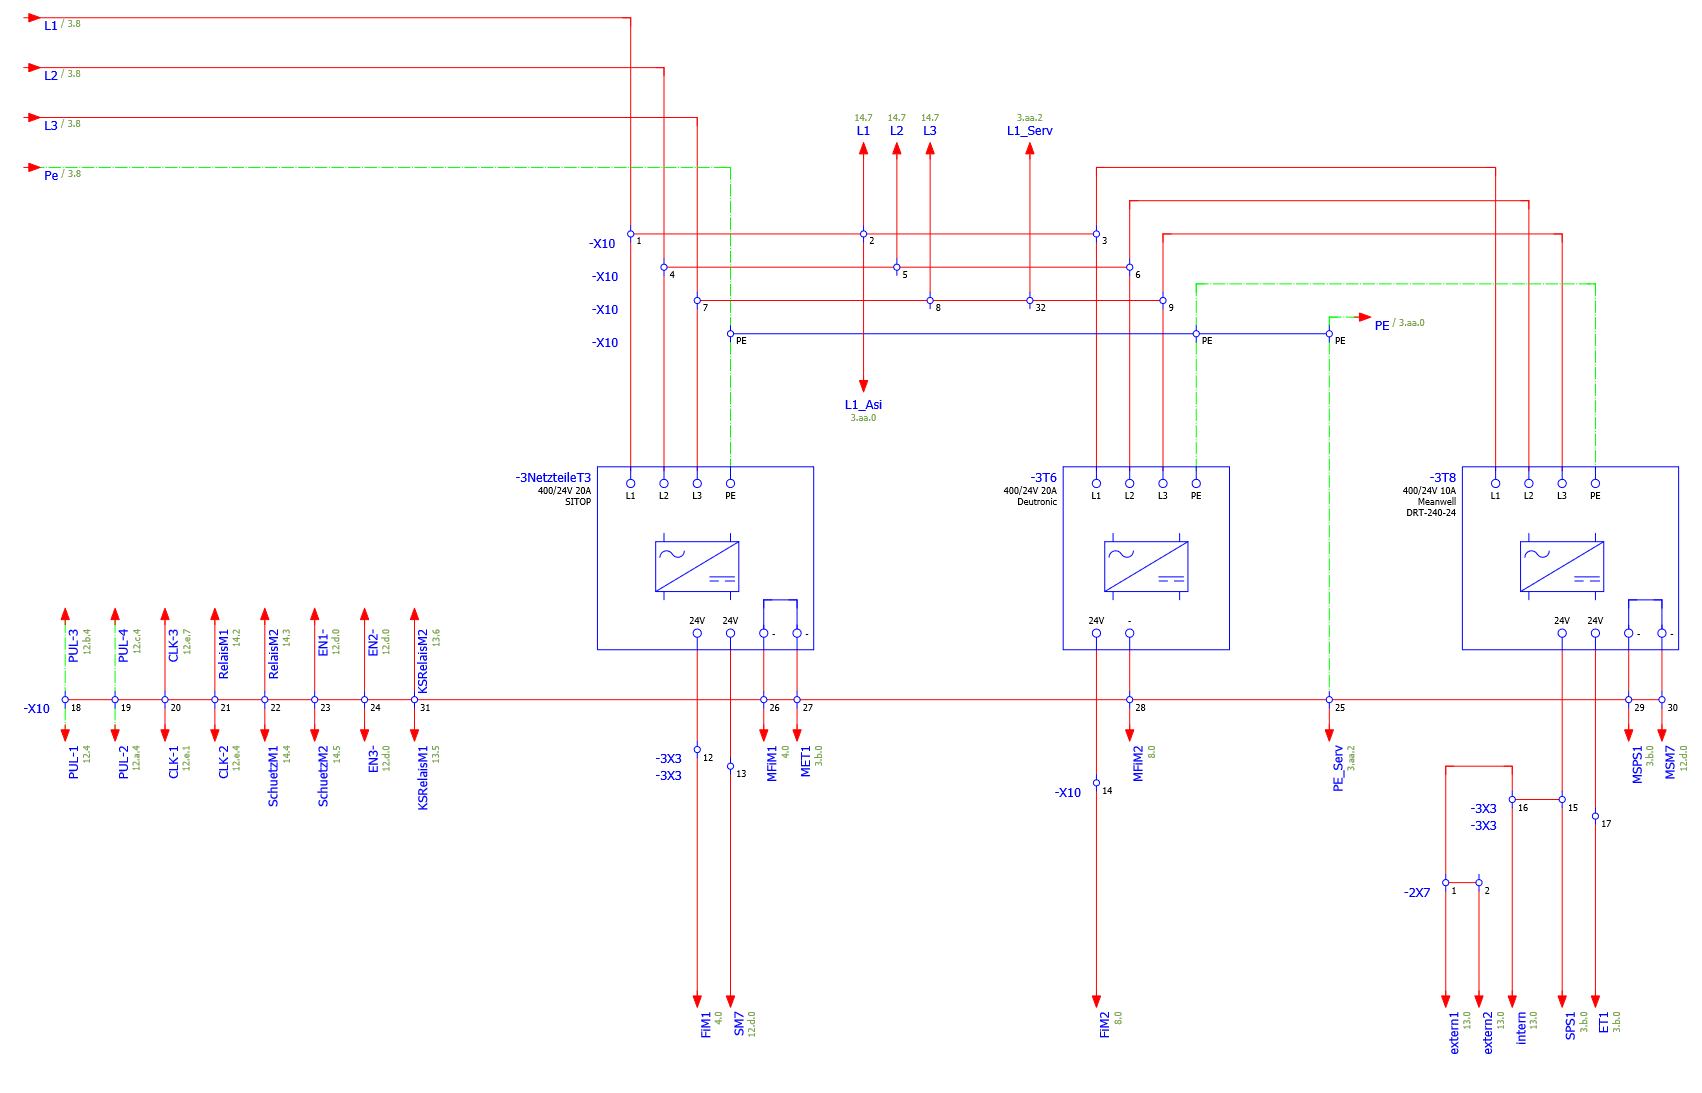
\includegraphics[width=0.9\textwidth]{Vogis Bilder/Netzteile_Schaltplan.png}
        \caption{Schaltplan: Netzteile}
        \label{fig:Netzteile}
    \end{figure}Was jetzt noch übergeblieben ist sind die 24V-DC-Minuspole der Netzteile. Die Reihenklemmen wurden über Querverbinder mitteinander zusammenverbunden und im Anschluss auch mit den PE-Klemmen der 230V Seite verbundnen. Die Entscheidung den Steuerstromkreis zu Erden beruht auf der Norm EN60204-1. Demnach hilft die Erdung gegen EMV-Probleme und gewährleistet im Fehlerfall die Abschalltung. \cite{elektronet_steuerstromkreis_geerdet}\cite{beckhoff_steuerstromkreis_geerdet}\\\\
    Die nächste Seite ist ein Nachtrag, denn anfänglich wurde nicht bedacht, dass der ASI-Kreis eine eignene 24V-DC-ASI-Versorgung braucht. Auf die zweite Seite wurde demnach die ASI-Versorgung gezeichnet sowie der Anschluss an den ET200-ASI-Master. Eingehend sind auf dieser Seite der L1, N und und ein Set, letzteres ist ein Eingang beim ASI-Master und wird von der SPS aus gesetzt, und ausgehend ist der ASI-BUS vom ASI-Master. Weiters befindet sich auf dieser Seite auch die Verdrahtung der Service Schnittstelle. Diese wird auch zusätzlich mit einem zweiphasigen Leitungsschutzschalter gesichert.\\\\
    Auf der dritten Seite wurde der Versorgungsanschluss von SPS und ET200 gezeichnet. Eingehend sind 24V einmal für die SPS sowie für die ET200 und der jeweilige Minuspol dazu. Auf dieser Seite wurden die Drahtverbindungen gezeichnet, die die SPS, die Ein und Ausgangskarten sowie die beiden PTO-Karten versorgt.\\\\
    Auf der vierten Seite findet sich das erste Feed-In-Modul von Weidmüller. Hierbei eingehend sind 24V, mit Minuspol, von der SITOP und ausgehend sind die Brückenverbindungen von den DC-Sicherungen. Das wären zwei mal Brücken für 24V, zwei mal Brücken für GND und eine Brücke für den BUS dieser Bugruppe.\\\\
    Auf den nächsten beiden Seiten finden sich jweils eine 8A-DC-Sicherung. Eingehend sind die bereits genannten Brücken, diese gehen dann auch weiter zur nächsten Sicherung, und ausgehend sind einmal + und - für die stärkeren Schrittmotoren. Wie erwähnt sind das Seite fünf und sechs.\\\\
    Auf Seite sieben findet sich eine 2A-DC-Sicherung für einen von drei schwächeren Schrittmotor. Diese hat ebenfalls die Brückenverbindung eingehend, allerdings hört die Brückenverbindung mot dieser Sicherung auf. Das bedeutet ein Feed-In-Modul versorgt drei Sicherungen. Abgehend hat diese Sicherung + und - für den passenden Schrittmotor.\\\\
    Ab der Seite acht wiederholen sich die letzten vier Seiten, mit dem Unterschied dass die gebrückte Versorgungsleitung nicht von der SITOP kommt, sonder von der Deutronic. Auf der Ersten ist damit wieder das Feed-In-Modul für die zweite Baugruppe. Somit hat man auf den drei folgendes Seiten drei DC-Sicherungen (8A, 8A, 2A), auf jeder Seite jeweils eine und von jeder Sicherung zwei Abgänge für die Schrittmotoren.\\\\
    Ab Seite 13 sind vier fast idente Schaltpläne. Der Grundaufbau ist immer gleich, man kommt mit der Versorgung von den Sicherungen und geht damit in die Schrittmotorkarte Type CL57C von Nanotec. Von den Treibern wurden dann Verbindungen zu einem Schrittmotor gezogen und zum zugehörigen Geber.\\
    Wenn wir diesen Teil des Schaltplanes von der Motorseite aus betrachten gibt es für den Motor die Anschlüsse A+, A-, B+, B-. Das sind die Anschlüsse für die zwei Pole eines Schrittmotores. Der Geber, welcher mit dem Motor über einen Welle kekoppelt ist, hat die Anschlüsse EB+, EB-, EA+, EA-  und für die Versorgung VCC und GND. Der Treiber CL57C hat Ausgänge die genau dieselbe Bezeichnung haben. Die gleichnnamigen Anschlüsse wurden miteinander verbunden. \\Da der Motor nicht im Schaltschrank sondern am Lagerregal verbaut wird muss vom Treiber zum Motor beziehungsweise Geber ein Kabel verlegt werden. Dies wiederum bedeuet, dass wir im Schaltschrank vom Treiber zuerst auf Reihenklemmen gehen und an diese Reihenklemmen dann die Kabel geklemmt werden. Für den Schrittmotoren wird ein 5 adriges Kabel (inklusive PE) verwendet mit der Kabelbezeichnung "ÖLFLEX® CLASSIC FD 810 CY 5G0,75". Der PE Leiter wird an die Erdung des Schaltschrankes angeklemmt und dieses Kabel hat, um die elektromagnetische Verträglichkeit zu gewährleisten, eine Schirmung. Die Schirmung muss, um zu funktionieren, an die Schaltschrank-Erdung gelegt werden, weil damit der Schirm eine Senke sein kann für die von den Leitern abgestrahlten elektromagnetischen Wellen. Das Kabel wird auf einer Ankerschiene mit der entsprechenden Zugentlastungsklemme, auf dem Erdungsmodul, nicht nur zugentlastet sondern auch geerdet. Dabei muss dann aber bedacht werden, dass die Klemme Kontakt zum Schirm haben muss, und die Ankerschiene geerdet sein muss. Der Schirm sowie die Erdung dessen wurde im Schaltplan hinzugefügt. \\
    Bezüglich den Motorkabeln wurde ebenfalls die Farbe der Adern bedacht. Während beim "ÖLFLEX® CLASSIC FD 810 CY 5G0,75" die Adern durchgängig nummeriert sind sind es die Adern des Schrittmotors nicht. Diese haben die Farben Schwarz, Grün, Rot und Blau. Da man beim Verdrahten nicht immer wissen kann welche Farbe zu welchem Anschluss führt, wurde auch dies im Schaltplan gezeichnet.\\Auch der Geber benötigt ein Kabel. Für diesen wurde auf Patch-Kabel gesetzt. Das achtadrige "FL CAT5 PATCH 10,0" bietet die Möglichkeit RJ45 Stecker zu verwenden. Diese befinden sich jeweils an den Enden und ersparen im Schaltschrank eine Menge Reihenklemmen, da man nur für die Buchse eine Aussparung bedenken muss. Vor allem im Entwicklungsprozess ist das komfortable An und Abstecken ein großer Vorteil aufgrund der Zeitersparnis. Aber auch im späteren Normalbetrieb ist es von Vorteil, bei zum Beispiel einer Umsiedelung des AFSS, die Kabel einfach abstecken zu können. Auch diese Kabel haben einen Schrim der über den RJ45 Stecker geerdet werden kann.\\
    Damit wäre die Kommunikation von Treiber, Motor und Geber gezeichent. Doch es gehört auch die Kommunikation zur SPS dazu. Der Treiber hat folgende Kontakte: PUL+, PUL-, DIR+, DIR-, ENA+, ENA- und ALM, BRK, COM-. Alle Anschlüsse mit einem - am Ende beschreiben den Minuspol zum jweiligen Gegenstück mit +. Da In unserem Fall alle + Kontakte von der selben SPS kommen und damit alle die selbe Spannung referenzieren können PUL-, DIR-, ENA- und COM- zusammengeschlossen werden und daraufhin zur Sammelschiene der Minuspole geklemmt werden. PUL+ steht für pulse und reguliert die Geschwindigkeit der Drehung,  DIR+ steht für direction und reguliert die Drehrichtung, ENA+ steht für enable und Ab Seite 13 sind vier fast idente Schaltpläne. Der Grundaufbau ist immer gleich, man kommt mit der Versorgung von den Sicherungen und geht damit in die Schrittmotorkarte Type CL57C von Nanotec. Von den Treibern wurden dann Verbindungen zu einem Schrittmotor gezogen und zum zugehörigen Geber.\\
    Wenn wir diesen Teil des Schaltplanes von der Motorseite aus betrachten gibt es für den Motor die Anschlüsse A+, A-, B+, B-. Das sind die Anschlüsse für die zwei Pole eines Schrittmotores. Der Geber, welcher mit dem Motor über einen Welle kekoppelt ist, hat die Anschlüsse EB+, EB-, EA+, EA-  und für die Versorgung VCC und GND. Der Treiber CL57C hat Ausgänge die genau dieselbe Bezeichnung haben. Die gleichnnamigen Anschlüsse wurden miteinander verbunden. \\
    Da der Motor nicht im Schaltschrank sondern am Lagerregal verbaut wird muss vom Treiber zum Motor beziehungsweise Geber ein Kabel verlegt werden. Dies wiederum bedeuet, dass wir im Schaltschrank vom Treiber zuerst auf Reihenklemmen gehen und an diese Reihenklemmen dann die Kabel geklemmt werden. Für den Schrittmotoren wird ein 5 adriges Kabel (inklusive PE) verwendet mit der Kabelbezeichnung "ÖLFLEX® CLASSIC FD 810 CY 5G0,75". Der PE Leiter wird an die Erdung des Schaltschrankes angeklemmt und dieses Kabel hat, um die elektromagnetische Verträglichkeit zu gewährleisten, eine Schirmung. Die Schirmung muss, um zu funktionieren, an die Schaltschrank-Erdung gelegt werden, weil damit der Schirm eine Senke sein kann für die von den Leitern abgestrahlten elektromagnetischen Wellen. Das Kabel wird auf einer Ankerschiene mit der entsprechenden Zugentlastungsklemme, auf dem Erdungsmodul, nicht nur zugentlastet sondern auch geerdet. Dabei muss dann aber bedacht werden, dass die Klemme Kontakt zum Schirm haben muss, und die Ankerschiene geerdet sein muss. Der Schirm sowie die Erdung dessen wurde im Schaltplan hinzugefügt.    
    \begin{figure}[h]
        \centering
        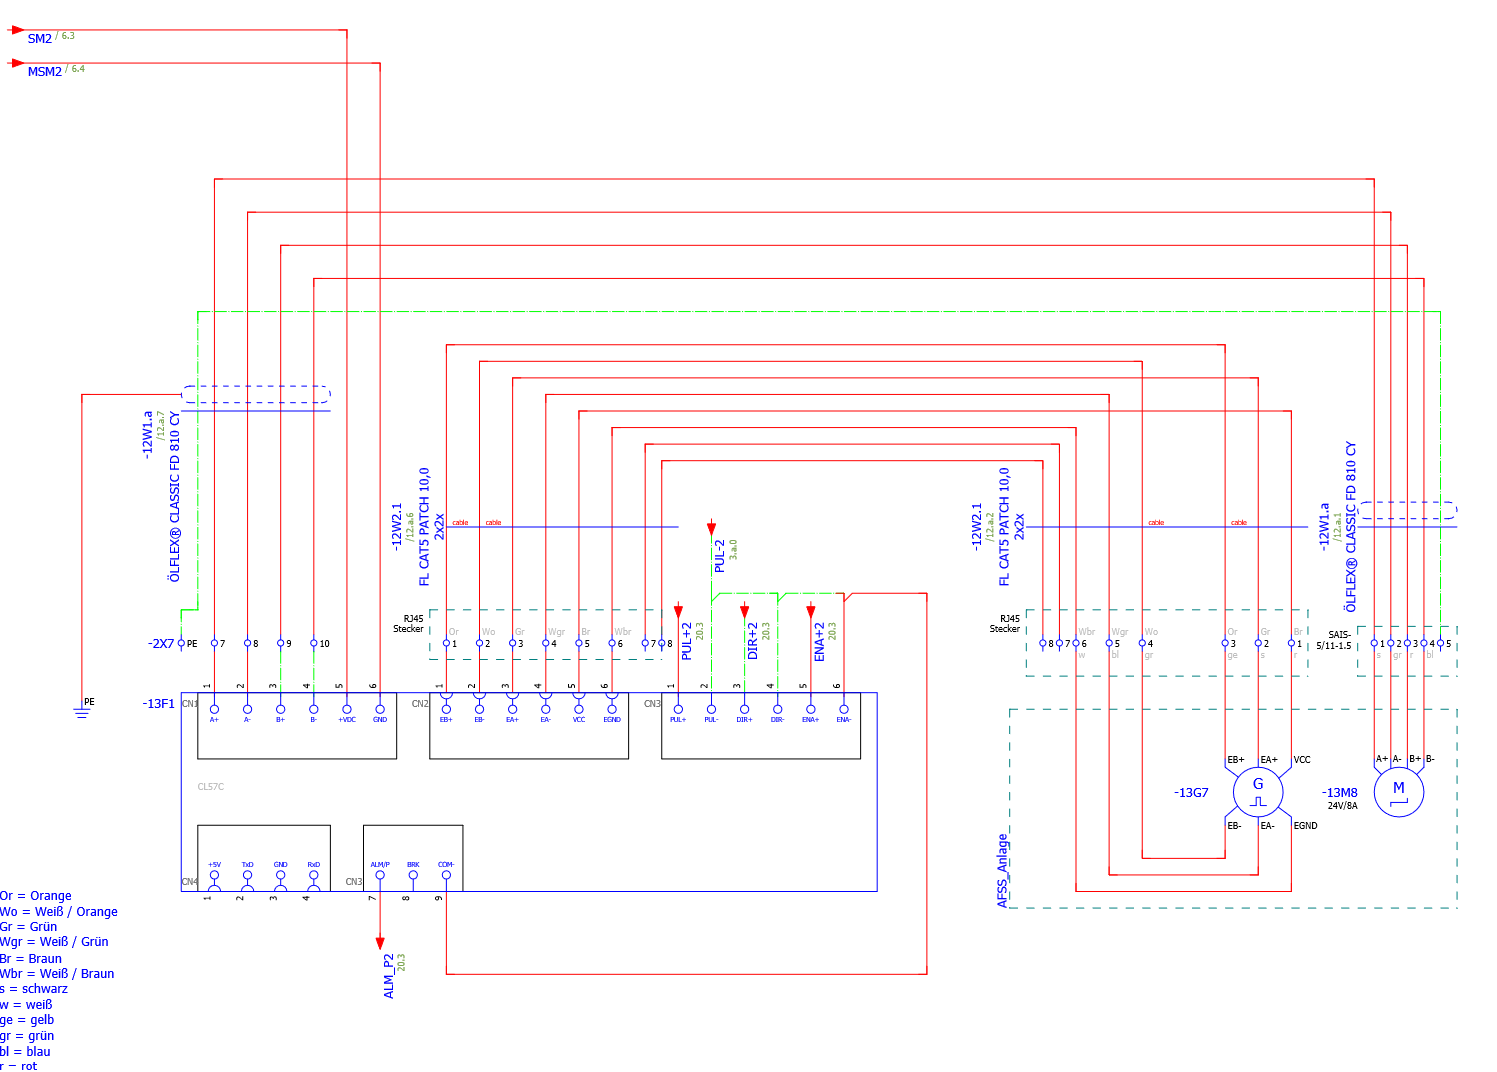
\includegraphics[width=0.9\textwidth]{Vogis Bilder/Schaltplan_SM1.png}
        \caption{13te Seite des Schaltplans, SM ohne Bremse}
        \label{fig:SMohneBremse}
    \end{figure}
    \\Bezüglich den Motorkabeln wurde ebenfalls die Farbe der Adern bedacht. Während beim "ÖLFLEX® CLASSIC FD 810 CY 5G0,75" die Adern durchgängig nummeriert sind sind es die Adern des Schrittmotors nicht. Diese haben die Farben Schwarz, Grün, Rot und Blau. Da man beim Verdrahten nicht immer wissen kann welche Farbe zu welchem Anschluss führt, wurde auch dies im Schaltplan gezeichnet.\cite{Nema_SM_Kontaktbezeichnung}\\
    Auch der Geber benötigt ein Kabel. Für diesen wurde auf Patch-Kabel gesetzt. Das achtadrige "FL CAT5 PATCH 10,0" bietet die Möglichkeit RJ45 Stecker zu verwenden. Diese befinden sich jeweils an den Enden und ersparen im Schaltschrank eine Menge Reihenklemmen, da man nur für die Buchse eine Aussparung bedenken muss. Vor allem im Entwicklungsprozess ist das komfortable An und Abstecken ein großer Vorteil aufgrund der Zeitersparnis. Aber auch im späteren Normalbetrieb ist es von Vorteil, bei zum Beispiel einer Umsiedelung des AFSS, die Kabel einfach abstecken zu können. Auch diese Kabel haben einen Schrim der über den RJ45 Stecker geerdet werden kann.\\
    Damit wäre die Kommunikation von Treiber, Motor und Geber gezeichent. Doch es gehört auch die Kommunikation zur SPS dazu. Der Treiber hat folgende Kontakte: PUL+, PUL-, DIR+, DIR-, ENA+, ENA- und ALM, BRK, COM-. Alle Anschlüsse mit einem - am Ende beschreiben den Minuspol zum jweiligen Gegenstück mit +. Da In unserem Fall alle + Kontakte von der selben SPS kommen und damit alle die selbe Spannung referenzieren können PUL-, DIR-, ENA- und COM- zusammengeschlossen werden und daraufhin zur Sammelschiene der Minuspole geklemmt werden. PUL+ steht für pulse und reguliert die Geschwindigkeit der Drehung,  DIR+ steht für direction und reguliert die Drehrichtung, ENA+ steht für enable und entsperrt den Treiber beziehungsweise gibt frei, dass ein Ansteuerung gewünscht ist. BRK steht für break und würde benötigt werden, wenn eine Bremse angedacht wäre, was sie in diesem Fall aber nicht ist. ALM steht für arlarm und ist ein Ausgang der einen erkannten Fehler meldet.\\
    ALM wurde mit der Eingangskarte verbunden und PUL+, DIR+ und ENA+ wurden an die zugehörigen Kontakte bei den PTO Karten der SPS gezeichnet.\\     
    \begin{figure}[h]
        \centering
        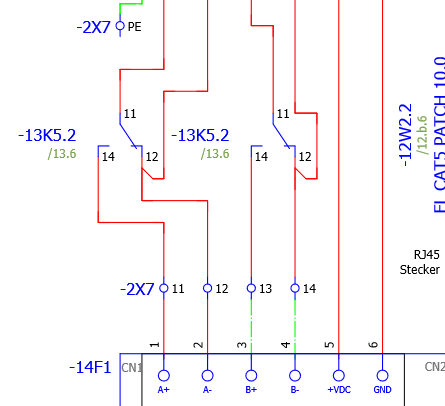
\includegraphics[width=0.5\textwidth]{Vogis Bilder/Schaltplan_SM_bremse.png}
        \caption{Zusätzliche Kurzschließung von Spulen bei horizontalen Antrieben}
        \label{fig:SMmitBrems}
    \end{figure}
    Während die ersten beiden SM-Treiber Schrittmotoren ansteuern die keine Bremsfunktion brauchen, da sie den Apparat nur horizontal bewegen und damit bei plötzlichem Ausfall, die Anlage auf dieser Achse zum Stillstand kommt, brauchen die anderen Zwei eine Bremsfunktion. Die zwei restlichen SM-Treiber steuern Motoren an, die zum Heben des Gabelapparates sind, uns wenn diese auf einmal ausfallen würden, würde die Schwerkraft das Konstrukt zu Boden fallen lassen. Deswegen sollen im Fehlerfall Relaiskontakte die Spulen der Schrittmotoren kurzschließen und damit eine bremsende Wirkung ermöglichen. Dabei funktioniert das Prinzip so, dass bei plötzicher Spannungsabwesenheit das Relais loslässt und die Spulen kurzgeschlossen sind. Das heißt im spannungsfreien Zustand sind die Spulen kurzgeschlossen siehe Abbildung \ref{fig:SMmitBremse}.\\\\ 
    Auf den darauf folgenden zwei Seiten befindet sich die Steuerung von den schwächeren Schrittmotoren. Auch diese haben Treiber und Motoren aber keine Geber.\\
    Auch die Geber für die schwächeren Schrittmotoren haben einen enable-Eingang. Dieser ist jedoch dann enabled wenn der Eingang Spannungsfrei ist. Aufgrund dieser Eigenschaft gibt es die Gefahr, dass die Schrittmotoren schneller losfahren als die SPS die Spannung aufgebaut hat. Beispielsweise wenn die Anlage einen Neustart durchführt könnte diese Situation entstehen. Deswegen werden die Eingänge Invertiert. Ein Relaiskontakt, ein Öffner, setzt den EN-Eingang immer auf 24V, erst sobald die SPS das Relais ansteuert kann der Treiber enabeled werden. Bei drei Treiber macht dies drei Relais. Auf der 17ten Seite befinden sich somit die Relais und deren Öffnerkontakte. Anfänglich wurden hier fälschlicher Weiße Schließer eingeplant, im Verlauf der Arbeit wurde diese Entscheidung hinterfragt und demnach auch ausgebessert. Auf der darauf folhgenden Seite finden sich die Treiber und Schrittmotoren.\\
    Zu den Treibern kann man sagen, dass alle Treiber ähnlich aufgebaut sind. Wieder gibt es einen Kontakt zur Geschwindigkeitsregelung (CLK+ und CLK-), einen zur Richtungsbestimmung (CW+ und CW-) und den bereits besprochenen Freigabeeingang (EN+ und EN-). Weiterführend haben die Treiber noch Anschlüsse für die Versorgungsspannung und A+, A-, B+ und B- für die Schrittmotoren. Die Massekontakte werden wieder alle zusammengeschlossen und weitergefürht zur gemeinsamen Masse.\\ 
    Auch für diese Motoren werden die selben Kabel verwendet wie zuvor. Wieder gilt, dass die Schirmung bei der Zugentlastung geerdet wird und auch die Farben der Adern wurden im Schaltplan eingezeichnet.\\
    \begin{figure}[h]
        \centering
        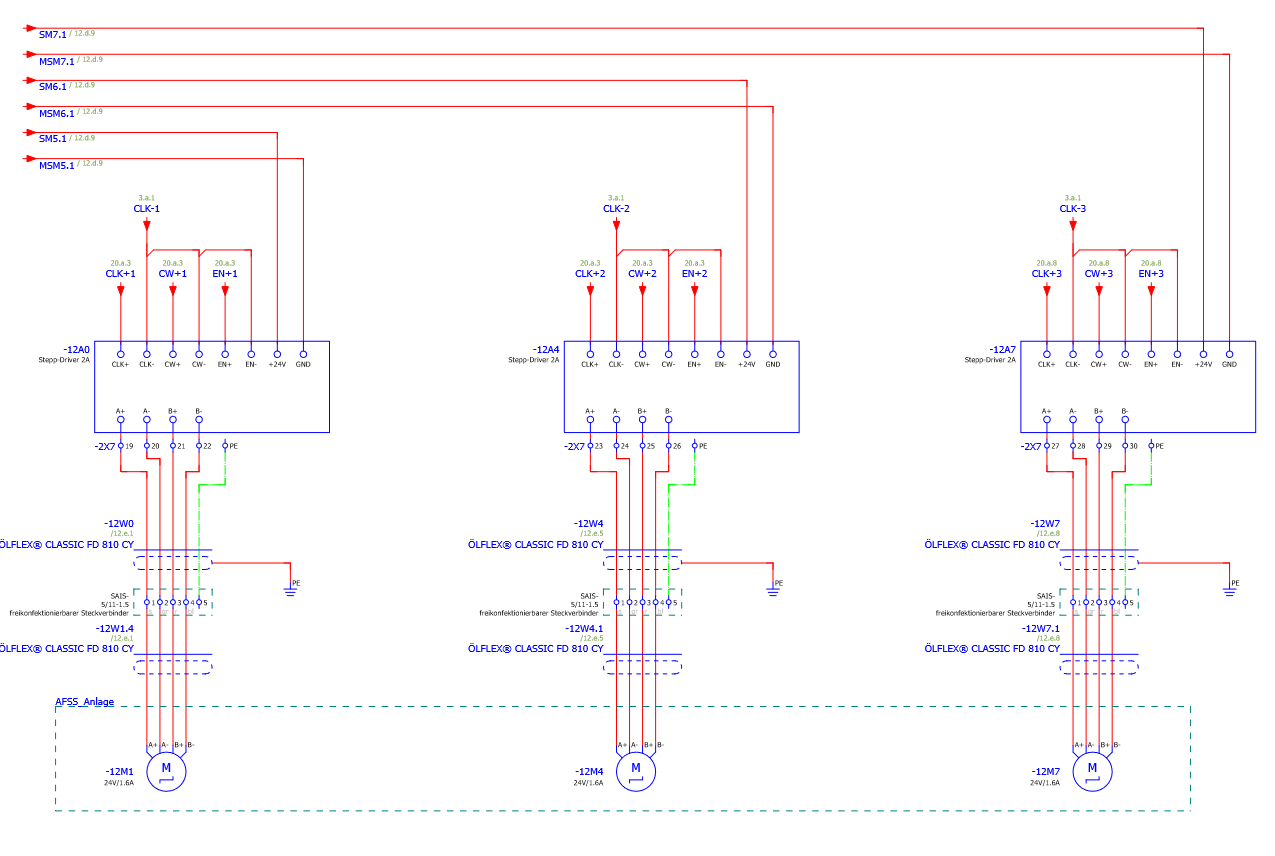
\includegraphics[width=0.9\textwidth]{Vogis Bilder/SM_Klein_Schaltplan.png}
        \caption{40Ncm Schrittmotoren im Schaltplan}
        \label{fig:SMkleine}
    \end{figure}
    Auch hier wurden die Steuerkontakte von den Treiben an die PTO-Karten der SPS angeschlossen.\\\\
    Auf der 19ten Seite befinden sich Not-Aus-Schaltungen und die Relais die dem Vertikalantrieb die Bremsfunjktion geben. In Summe sind es vier Not-Aus und zusätzlich noch ein Schlüsselschalter zur Freigabe. Für die fünf Sensoren gibt es drei Versorgungsleitungen, je nach räumlicher Position teilen sich die Komponenten eine Leitung, und alle haben jeweils einen Abgang zur SPS-Eingangskarte. Die Relais bekommen ihre Versorgung von der SPS und haben Abgänge zur gemeinsamen Masse. Die Funktion der Relais wurde bereits beschrieben.\\\\ 
    Die nächste Seite zeigt die ganze Steuerung des Asynchromotors, welcher das Förderband antreibt. Hierfür gibt es Schütz die in einer Wendeschützschaltung den Asynchronmotor ansteuern. Es ist keine Drehzahlregelung nötig. Die Schütze blockieren sich gegenseitig und werden angesteuert über zwei Relais. Diese Relais werden direkt von der SPS angesteuert. Beim Asynchronmotor gibt es noch einen Motorschutzschalter, dessen genauere Auslegung im Verlauf der Diplomarbeit noch genauer beschrieben wird.\\\\
    Die Seiten 21 und 22 zeigen die PTO-Karten der SPS. PTO steht Pulse-Train-Output und steuert die Treiber an. Ursprünglich wären für diese Aufgaben PWM-Karten von Weidmüller verwendet worden, es ist allerdings bei Testversuchen aufgefallen, dass diese nicht in der Lage sind variable Frequenzen zu erzeugen. Damit musst eine Alternative her. Die Siemens PTO-Karten sind fähig die Frequenzen auch während dem Betrieb zu ändern und damit ermöglichen sie sanftes Anfahren der Schrittmotoren.Eine PTO-Karte kann vier Schrittmotoren steuern.\\
    Diese Karten haben mehrere Ausgänge und Eingänge. Im Fall des AFSS gehen vier mal die PUL+ und DIR+ und ENA+ aus und eingehend sind die vier ALM (Arlarmmeldungen). Das sind die Kontakte von den vier stärkeren Treibern und damit ist die erste PTO-Karte voll ausgenutzt. Mit der Zweiten werden die Drei schwächeren Treiber angesteuert. Diese mal wieder mit den unterschiedlich benannten Kontakten.\\\\
    Auf der folgendnen Seite befindet sich die Eingangskarte der SPS mit den Eingängen. Dabei werden primär die Zustände der Not-Aus-Schalter abgefragt und die des Schlüsselfreigabeschalters.\\\\
    Auf der Seite 24 befindet sich die Ausgangskarte der Siemens SPS. Mit dieser werden ausschließlich nur Relais angesteuert. Diese sind für die Invertierung der Enable-Eingänge der Treiber zuständig, für das Steuern der Schütze für den Asynchronmotor und zuletzt auch für die Bremsfunktion. Damit ist die Schaltung zur Steuerung aller Schrittmotoren fertig. Auf den folgenden Seiten wurde dann die Schaltung der ASI-Sensoren gezeichnet\\\\ 
    Bezüglich dem ASI-Netzt ist zu wiederholen, dass der ASI-Master mit den Slaves über einen zweiadrigen ASI-Bus kommuniziert. Für diesen Bus gibt es ein eigenes Kabel, aber da mit dem Material gearbeitet werden muss, was vorhanden ist wird beim AFSS das selbe fünf adrige Ölflex verwendet wie für die Motoren. In diesem ungünstigen Fall werden von den fünf adern am Ende nur zwei verwendet.\\
    \begin{figure}[h]
        \centering
        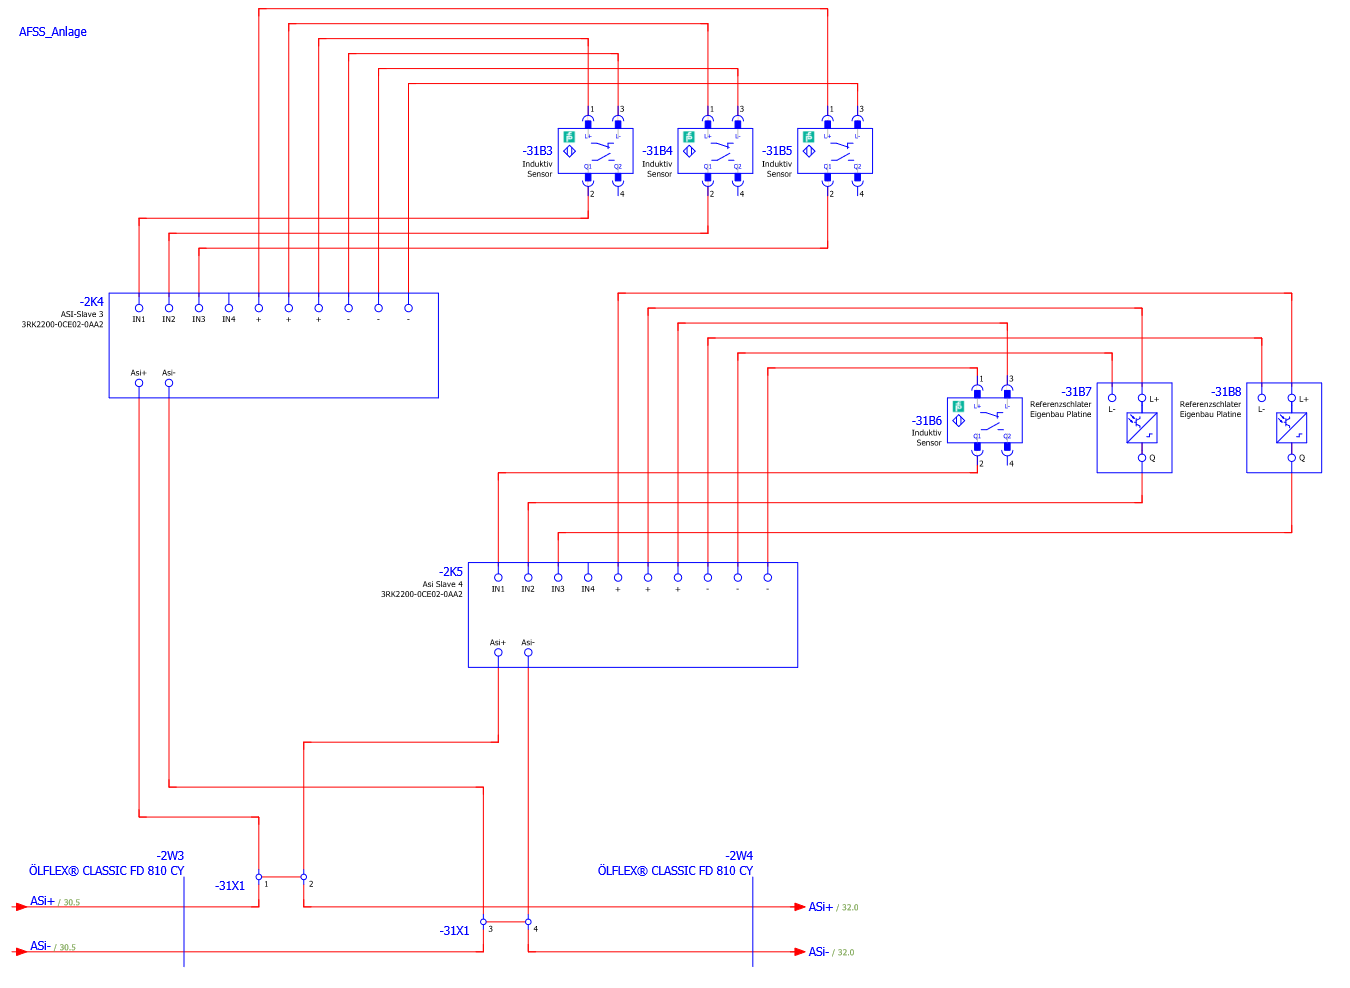
\includegraphics[width=0.9\textwidth]{Vogis Bilder/ASI_Schaltplan_sensoren.png}
        \caption{Sensoren mit den ASI-Slaves, erste Seite von vier}
        \label{fig:ASI_Sensoren}
    \end{figure}
    Bezüglich den Slaves ist zu sagen, dass ursprünglich ein Slave mit sieben Inputs gedacht. Dieser wäre in der Schule genügend vorhanden gewesen. Allerdings ist bei Testläufen es nicht gelungen eine Kommunikation zwischen diesen Slaves und dem Siemens ASI-Master herzustellen. Deswegen werden anstatt vier Slaves mit sieben Eingängen nun sieben ASI-Slaves von Siemens mit jeweils vier Eingängen verwendet. Der genaue Typ ist 3RK2200-0CE02-0AA2 und es ist möglich mit diesem zu kommunizieren.\\
    Der Bus fährt auf mit Steckverbinder erweiternde Reihenklemmen, von denen dann auf die jeweiligen Slaves. Es sind immer zwei Slaves räumlich beieinander und werden gemeinsam mit Reihenklemmen auf dem AFSS auf Hutschienen montiert. Der siebte Slave ist alleine. Wie die Sensoren mit den ASI-Slaves verbunden sind sieht man auf der Abbildung \ref{fig:ASI_Sensoren} und für eine genaue Erklärung zu den Sensoren siehe Kapitel \ref{sec:Sensorik}.\\
    In Summe erstreckt sich der genaue Schaltplan der ASI-Slaves über die letzten vier Seiten.
    \paragraph{Topologieansichten}\mbox{}\\
    Nachdem alle Seiten gezeichnet und überarbeitet wurden, wurden für den ASI-Bus und den PROFIBUS noch passende Topologieansichten gezeichnet. Diese bieten eine übersichtliche Darstellung der Buse.
    \paragraph{Übersichtsblätter}\mbox{}\\
    Daraufhin wurden noch zwei Übersichtsblätter gezeichnet. Auf diesen ist die gewünschte Anreihung der Siemens SPS und ihren Karten sowie der ET200 mit ihrem ASI-Master.
\subsection{Die Auslegung verschiedenster Schaltschrankkomponeten}
    \paragraph{Fehlerstomschutzschalter}\mbox{}\\
    Der FI ist ein Schutzorgan, welches im Fehlerfall den Stromkreis unterbricht. Dieser erkennt wenn der Summenstrom von L1, L2, L3 und N nicht mehr gleich Null ist und schaltet dann ab.\\
    Beim FI gibt es verschiedenste Arten. Die älteste wäre der TYP AC, es gibt aber auch noch TYP A, B und F sowie Weitere. Von den genannten Typen wurde für das AFSS ein Fehlerstromschutzschalter der Variante A gewählt, da bei dieser Anlage das erkennen von Wechselströmen und Pulsströmen genügt. Das liegt daran, dass kein Spezialfall vorliegt, der einen anderen Typen fordern würde \cite{FI-Typen}.
    \paragraph{Leitungsschutzschalter}\mbox{}\\
    Beim Leitungsschutzschalter gibt es die Schaltcharakteristik sowie den Bemessungsstrom der gewählt gehört. Da im AFSS die ASM zu hochen Anlaufströmen führt wurde Charakteristik des Typs C gewählt, dieser ist anzuwenden in Schaltkreisen mit Motoren oder Handwerkzeug \cite{SeyrRösch}. Für den Bemessungsstrom wurde 13 A ausgewählt, da dieser Wert der nächsthöhere zum Nennstrom war. Der Nennstrom wurde ermittelt aus der Summe der einzelnen Nennströme der Verbraucher multipliziert mit einem Gleichzeitigkeitsfaktor. Bei letzterem Faktor wurde geschätzt wie viele Verbraucher gleichzeitig laufen werden. Die Gabel-Antriebe beispielsweise werden nie gleichzeitig zu irgendeinem anderem Motor ein oder ausfahren. 
    \paragraph{Motorschutzschalter}\mbox{}\\
    Der Asynchromotor hat im Falle des AFSS einen Nennstrom von 1,9 A. Beim AFSS wird ein Standardmotorschutzschalter verwendet, der auf den Nennstrom des Motors angepasst wurde. 
    \paragraph{Leiterquerschnitte}\mbox{}\\
    Der Leiterquerschnitt ist abhängig vom Spannungsabfall, der aufgrund von kurzen Längen im Schaltschrank irrelevant ist, von Verlegeart und Nennstrom. Der Leiterquerschnitt hängt auch immer mit den Sicherungselementen zusammen, da der Leiter so lange den Strömen standhalten muss, bis das Schutzelement ausgelöst hat. Deswegen wird im AFSS ein Leiterquerschnitt von 2,5 mm² verwendet, bis zu entsprechenden Sicherheitslementen und von dort aus wird dann auf 0,75 mm² reduziert \cite{SeyrRösch}.\\ 
    Alle Erdungskontakte werden mit 2,5 mm² verdrahtet um alle potentiellen Fehlerströme auszuhalten.\\
    Die Farben der einzelnen Drähte werden mit dem Schulinternen Standard entschieden beziehungsweise festgelegt.
\subsection{Realisierung}
    Nach der Planung kommt die Realisierung des Geplanten. Bei dieser gibt es mehrere Schritte. Diese werden nun näher beleuchtet.
    \paragraph{Rädermontage}\mbox{}\\
    Der erste Schritt vom Serverschrank zum Schaltschrank des AFSS war die Mobilmachung. Dem Serverschrank wurden vier Räder in den unteren Ecken gegeben. Dafür wurden in den bestehenden Boden für jedes Rad vier Löcher manuell gebohrt. Die Räder wurden daraufhin mit Schrauben, Beilegscheiben und Muttern montiert.\\
    Bei den Rädern handelt es sich um Zwei fixierte und Zwei die sich um 360° drehen können. Wichtig war, dass sich ein Paar nicht diagonal zueinander sondern nebeneinander montiert wird. Wären die Flexiblen diagonal zueinander könnnte man mit dem Schaltschrank im besten Fall nur in eine Richtung fahren. Angeordnet wurden die Räder vergleichbar zu einem Einkaufswagen.  
    \paragraph{Filou-NC}\mbox{}\\
    Nachdem die Module in AutoCAD neugezeichnet (siehe Abschnitt \ref{AutoCAD}) wurden, konnten die DXF-Dateien in Filou-NC importiert werden.\\
    In Filou-NC wird die gesammte DXF-Datei importiert. Danach kann man unerwünschte Teile der Zeichnung löschen, wenn beispielsweise mehrere Module in der selben Zeichnung vorhanden sind müssen die, die nicht gefräst werden gelöscht werden. Daraufhin sollte die Zeichnung noch bereinigt werden, das heißt, dass doppelte Linien gelöscht werden. Das Programm liefert hierfür ein fertiges Tool. Gewisse Längen der Zeichnung müssen nun noch unterbrochen werden. Das dient dazu, dass beim Fräsvorgang die Platte immer zumindest an den Unterbrechungen mit der ursprünglichen Platte verbunden bleibt. Verhindert wird, dass sich die Platte verschiebt und somit nicht mehr an den richtigen Stellen gefräst wird.\\
    Nachdem die DXF-Zeichnung vorbereitet wurde muss nun der Fräsablauf programmiert werden. Dazu muss im Programm dem Ablauf ein Startpunkt vergeben werden und der Nullpunkt der Zeichnung gesetzt werden. Daraufhin kann man das in echt eingespannte Werkzeug auch digital im Programm einfügen. Damit das Programm weiß wie groß der Durchmesser des Werkzeuges ist und wie die Spitze des Werkzeuges aussieht. Nachdem das Werkzeug eingefügt wurde ist die Sprühdüse, zur Kühlung, einzuschalten und daraufhin kann man die Konturen der Zeichnung mit dem Werkzeug abfahren. Beim festlegen der Fräsbahnen ist darauf zu achten, dass die richtige Anzahl an Zustellungen eigestellt wurde. Zustellungen legen fest, dass nicht die ganze Dicke des Materials auf einmal abgetragen werden. Bei dickerem Material ist dies nötig um das Werkzeug zu schützen.\\
    Wenn diese Schritte erfogleich ausgeführt wurden kann ein NC-Code exportiert werden. 
    \paragraph{Fräsen}\mbox{}\\
    Der genannte NC-Code kann nun auf die CNC-Fräse geladen werden. Bei der Fräse ist nun noch der Nullpunkt zu setzen und die Werkzeuglänge zu kalibrieren. Bei der Nullpunktsetzung ist es wichtig zu beachten, dass keines der Spannelemente, die die Platte auf den Frästisch fixieren, beim fräsen im Weg sein wird.\\
    Daraufhin kann der Fräsvorgang gestartet werden. Währenddessen ist zu beachten, dass bei der Sprühdüse genügend Flüssigkeit rauskommt, da dies manuell einzustellen ist. Ebenfalls ist das Werkzeug zu beobachten, ob unerwartete Ereignisse auftretten, beispielsweise Rauch oder Dampfbildung.\\ 
    Nach einem gelungenen Fräsvorgang wird die gesammte Fräse gereinigt und die Platte entnommen.\\
    Im angewandten Fall des AFSS wurde zu erst nur ein Modul gefräst und vollständig fertiggestellt, damit festgestellt werden kann, ob die Maße stimmen. Das erste Modul passte und danach wurden alle verbleibenden Platten an zwei Tagen gefräst.

    \paragraph{Fräsen-Nachbearbeitung}\mbox{}\\
    Nachdem die Platte von der Fräse genommen wurde, hat diese viele scharfe Kanten. Diese werden mit entspechendem Werkzeug entgratet. Rückstände von der Kühlflüssigkeit oder Kunststoff beziehungsweise Metallspäne wurden sorgfältig abgewischt.
    \paragraph{Module-Fertigstellung}\mbox{}\\
    Den Module müssen nun bestückt werden. Dazu wurden die Profilschinen und Montagekanäle abgelängt und mit M5 Schrauben und Muttern montiert.\\
    Die Elemente die nicht auf Profilschienen montiert werden, wurden mit den für das jeweilige Elemt vorgesehenen Schrauben und Muttern montiert.\\
    Auf die gennanten Profilschinen (Siemens oder Hutschiene) wurden noch die passenden Elemnte aufgesteckt.\\
    Die Platten konnten nun in den Schaltschrank, auf die vorhandenen Schienen montiert werden. Doch diese mussten zuvor nach innen versetzt werden. 
    \begin{figure}[h]
        \centering
        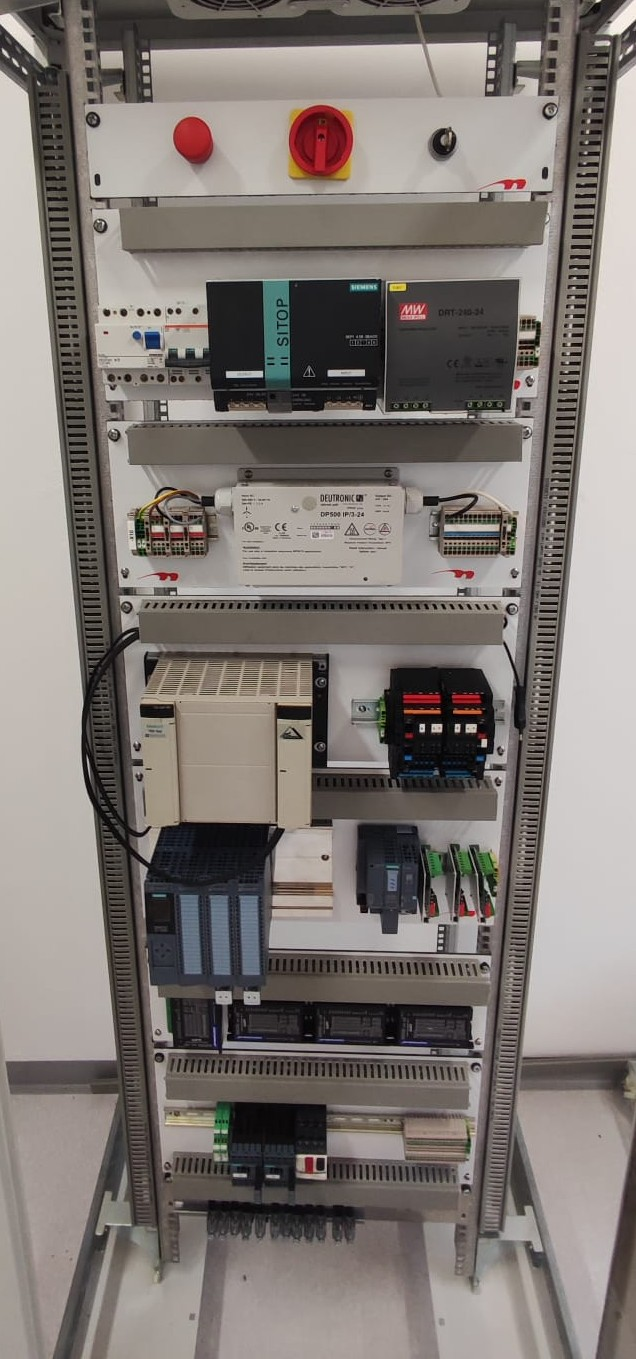
\includegraphics[width=0.3\textwidth]{Vogis Bilder/Schaltschrank_only_module.jpg}
        \caption{Schaltschrank mit eingebauten Modulen}
        \label{fig:Schaltschrank_onlyModule}
    \end{figure}    
    \paragraph{Profilschienen-Verschiebung}\mbox{}\\
    Zwei Profilschienen wurden um ca. 300 mm nach innen versetzt. Dafür wurden die Winkel, die die Profilschienen an den Serverschrank befestigten, gelöst und weiter innen neu montiert. Das war deswegen möglich, da die Winkel an einer weiteren Profilschiene montiert waren. Diese bisher nicht gennate Profilschiene besteht im Schaltschrank vier mal und ist oben und unten quer befestigt (siehe Abildung \ref{fig:Clean_Serverschrank}). Nachdem dieser Schritt gemacht wurde konnten die Modulplatten an die verschobenen Profilschienen geschraubt werden (Schaltschrank ohne verdrahtung siehe Abbildung \ref{fig:Schaltschrank_onlyModule}).  
    \paragraph{Folierung der Frontscheibe}\mbox{}\\
    Da der Schaltschrank des AFSS mobil ist, wurde entschieden, dass auch für nicht eingeweihte Personen stehts klar sein soll, wessen Schaltschrank dies ist. Dafür wurde der Schaltschrank mit einer Folierung versehen. Auf dieser ist sind die Teammitglieder aufgelistet, unter anderem FL. Wurnitsch, damit ist die Zugehörigkeit deutlich gekennzeichnet (siehe Abbildung \ref{fig:Schaltschrank_foliert}). Die Folierung wurde mit Hilfe der in der Schule vorhandenen Stickerschneidemaschine gemacht.
    \begin{figure}[h]
        \centering
        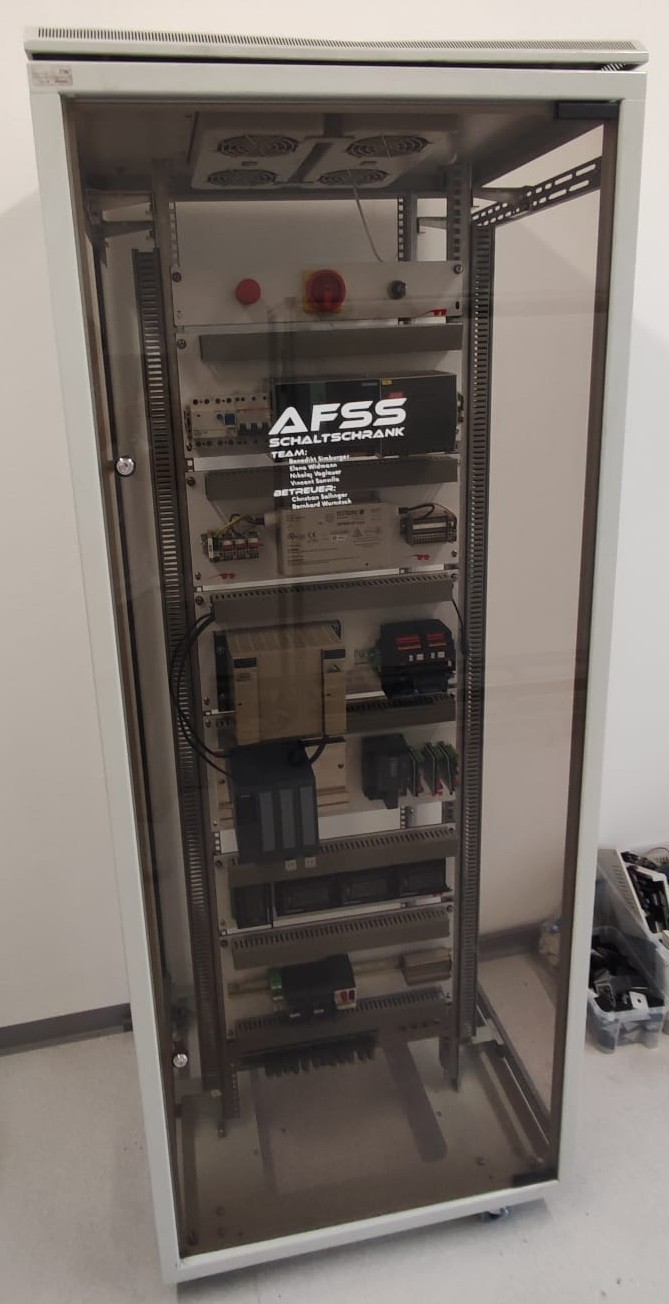
\includegraphics[width=0.3\textwidth]{Vogis Bilder/Schaltschrank_foliert.jpg}
        \caption{Schaltschrank mit Folierung}
        \label{fig:Schaltschrank_foliert}
    \end{figure}
    \paragraph{Die Verdrahtung}\mbox{}\\
    Nachem alle Modifikationen am Serverschrank vollzogen waren und alle Module eingebaut waren war die Transformation vom Serverschrank zum Schaltschrank fast vollzogen. Es fehlte noch die Verdrahtung.\\
    Zu dieser ist zu sagen, dass eine vollständige Verdrahtung der ganzen Anlage sich zeitlich nicht ausgegangen hätte. Deswegen wurde sich auf einen Kompromiss geeinigt. Dieser besagt, dass genügend verdrahtet wird, sodass die X-Achse ansteuerbar ist.\\
    Beim Verdrahten wurden die bereits gennanten Querschnitte beachtet aber auch die schulinterne Leitinie zur Drahtfarbe im Schaltschrank wurde beachtet. Diese besagt: Rot für Versorgungen, Blau für Minus, Gelb für Ausgänge, von beispielsweise der SPS, und Orange für Eingänge, von  beispielsweiseSensoren.\\
    Beim Verdrahten wird unweigerlich der Schaltplan wieder und wieder durchdacht. Dabei fallen Fehler oder Verbesserungsmöglichkeiten schnell auf. Auch beim Verdrahten des Schaltschrankes des AFSS sind Fehler und Verbesserungspotentialle aufgefallen, beispielsweise, dass die Adern der Encoder-Kabel zwar Farben hatten, diese aber nicht am Schaltplan zugeteilt werden. Ein anderes Beispiel wäre, dass bei den PTO Module alle Eingänge verschoben waren. Diese und weitere Punkte wurden unverzüglich nachgebessert beziehungsweise hinzugezeichnet.\\
    \begin{figure}[h]
        \centering
        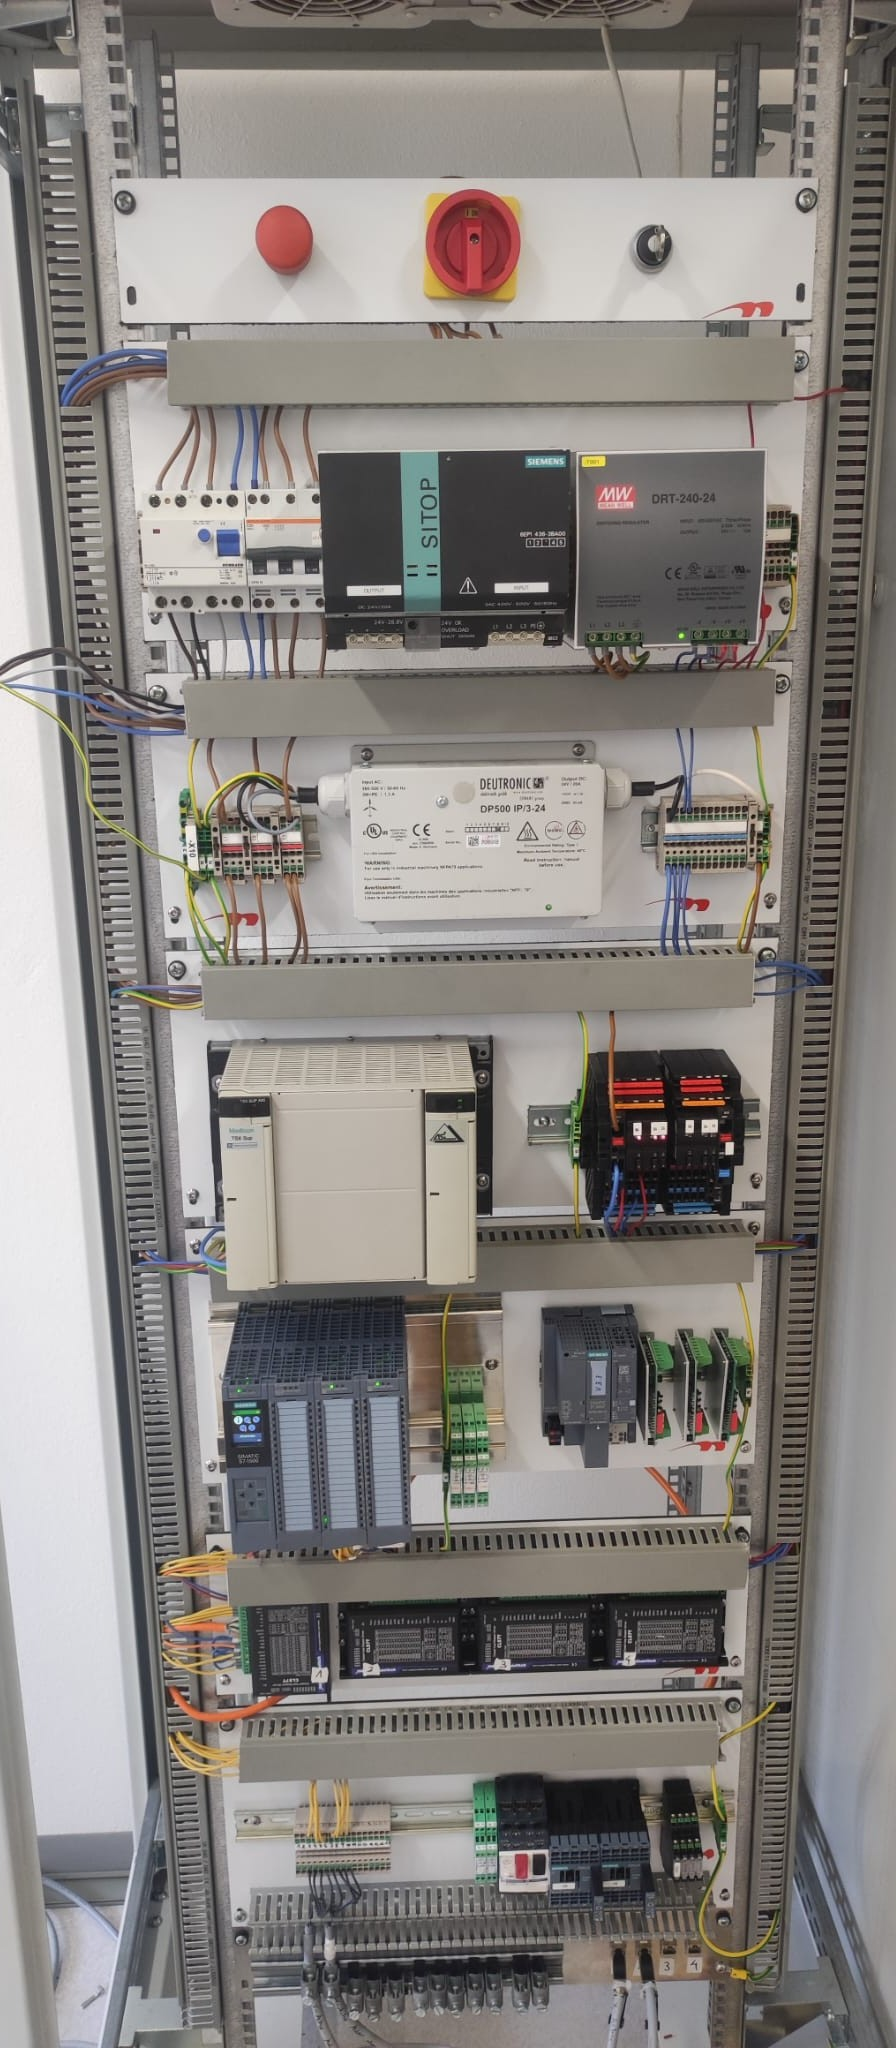
\includegraphics[width=0.3\textwidth]{Vogis Bilder/Schaltschrank_verkabelt.jpg}
        \caption{Schaltschrank mit Verdrahtung}
        \label{fig:Schaltschrank_verkabelt}
    \end{figure}
    \paragraph{Einbau von Service-Schnittstelle}\mbox{}\\ 
    Als letzte Modifikation wurde eine Service-Schnittstelle von Weidmüller in die rechte Metalwand des Schaltschrankes eingebaut. Dazu wurden manuell auf die Seitenwand die Maße angezeichnet die ausgeschnitten gehören. Entlang dieser Markierungen wurd daraufhin, unter beachtung aller dafür notwendigen Schutzmaßnahmen, mit einem Winkelschleifer geschnitten. Dieser hatte für das Schneiden von Metall dieser Stärke den entsprechenden Aufsatz. 
\subsection{Fazit}\mbox{}\\




